% **************************************************
% Information and Commands for Reuse
% **************************************************
\newcommand{\thesisTitle}{Migration von REST nach GraphQL in einer bestehenden Webapplikation}
\newcommand{\thesisSubtitle}{Bachelor-Thesis im Fachbereich Informatik}
\newcommand{\thesisDate}{09. September 2020}
%\newcommand{\thesisVersion}{\input{GIT_REV}}

\newcommand{\thesisAuthor}{Yannick Schröder}
\newcommand{\thesisAuthorStudentNumber}{Informatik 102751}
\newcommand{\thesisAuthorEmail}{inf102751@fh-wedel.de}

\newcommand{\thesisFirstReviewer}{Dr. Michael Predeschly}
\newcommand{\thesisFirstReviewerEmail}{\protect{mpr@fh-wedel.de}}

\newcommand{\thesisSecondReviewer}{M.~Sc. Marcus Riemer}
\newcommand{\thesisSecondReviewerEmail}{\protect{mri@fh-wedel.de}}

\newcommand{\thesisUniversity}{\protect{Fachhochschule Wedel}}
\newcommand{\thesisUniversityCity}{Wedel}
\newcommand{\thesisUniversityStreetAddress}{Feldstra{\ss}e 143}
\newcommand{\thesisUniversityPostalCode}{22880}



% **************************************************
% Load and Configure Packages
% **************************************************
\usepackage[utf8]{inputenc}       % defines file's character encoding
\usepackage[ngerman]{babel}       % babel system, adjust the language of the content
\usepackage[                      % clean thesis style
	figuresep=colon,%
	sansserif=false,%
	hangfigurecaption=false,%
	hangsection=false,%
	hangsubsection=false,%
	colorize=full,%
	colortheme=bluemagenta,%
	bibsys=bibtex,%
	bibfile=bib-refs,%
	bibstyle=alphabetic,%
]{sty/cleanthesis}

\hypersetup{                      % setup the hyperref-package options
	pdftitle={\thesisTitle},      %   - title (PDF meta)
	pdfsubject={\thesisSubtitle}, %   - subject (PDF meta)
	pdfauthor={\thesisAuthor},    %   - author (PDF meta)
	plainpages=false,             %   -
	colorlinks=false,             %   - colorize links?
	pdfborder={0 0 0},            %   -
	breaklinks=true,              %   - allow line break inside links
	bookmarksnumbered=true,       %
	bookmarksopen=true            %
}

% Font and Color
\cthesissetcolor{cmyk}{1, .87, .27, .12}{1, .87, .27, .12}
\usepackage{fontspec}

% \setmainfont{Dax Pro}
% \renewcommand{\helv}{\fontspec{Dax Pro}\fontsize{12}{14}\selectfont}
% \renewcommand{\book}{\fontspec{Dax Pro}\fontsize{12}{14}\selectfont}
% \renewcommand{\tgherosfont}{\fontspec{Dax Pro}}
% \renewcommand{\thesischapterfont}{\color{ctcolorblack}\huge\fontspec{Dax Pro}}

% \renewcommand{\ttfamily}{\fontspec{Ubuntu Mono}}

\renewcommand{\cftchapfont}{\normalfont\bfseries}
\renewcommand{\cftchappagefont}{\normalfont\bfseries}
\usepackage{multicol}
\addtokomafont{caption}{\normalfont}
\addtokomafont{captionlabel}{\normalfont}
\urlstyle{rm}
\makeatletter
\def\blx@maxline{77}
\makeatother

\usepackage{hyperref}
\usepackage{nameref}

\makeatletter
\let\orgdescriptionlabel\descriptionlabel
\renewcommand*{\descriptionlabel}[1]{%
	\let\orglabel\label
	\let\label\@gobble
	\phantomsection
	%\edef\@currentlabel{#1}%
    \edef\@currentlabelname{#1}%
	\let\label\orglabel
	\orgdescriptionlabel{#1}%
}
\makeatother

% **************************************************
% Additional Utilities
% **************************************************

\newcommand{\fullref}[1]{\ref{#1}~\enquote{\nameref{#1}}}


% \inlinec for inline code
\NewDocumentCommand{\inlinec}{v}{%
\texttt{#1}%
}

% Fix quotes
\usepackage{csquotes}
\MakeOuterQuote{"}

% Code
\usepackage{listings,lstautogobble}

\definecolor{lightgray}{rgb}{.9,.9,.9}
\definecolor{darkgray}{rgb}{.4,.4,.4}
\definecolor{purple}{rgb}{0.65, 0.12, 0.82}
\definecolor{orange}{rgb}{1, 0.722, 0.424}

\lstset{
	numberstyle=\tiny
}


\lstdefinelanguage{SQL}{
	keywords={INSERT, UPDATE, DELETE, SELECT, FROM, WHERE, GROUP BY, SET, INTO, VALUES, LIMIT},
	keywordstyle=\color{blue}\bfseries,
	ndkeywords={strftime},
	ndkeywordstyle=\color{OliveGreen}\bfseries,
	identifierstyle=\color{black},
	sensitive=false,
	comment=[l]{//},
	morecomment=[s]{/*}{*/},
	commentstyle=\color{purple}\ttfamily,
	stringstyle=\color{red}\ttfamily,
	morestring=[b]',
	morestring=[b]"
}

\lstdefinelanguage{HTML}{
	keywords={select, option, h1, template, h2, div, ul, li, table, thead, tr, th, td, tbody, tr, value, innerHtml, class, id},
	keywordstyle=\color{blue}\bfseries,
	ndkeywords={for, in, include, endfor, endif, else, if, ngIf, ngFor, each},
ndkeywordstyle=\color{OliveGreen}\bfseries,
	identifierstyle=\color{black},
	sensitive=false,
	comment=[l]{//},
	morecomment=[s]{/*}{*/},
	commentstyle=\color{purple}\ttfamily,
	stringstyle=\color{red}\ttfamily,
	morestring=[b]',
	morestring=[b]"
}

\lstdefinelanguage{JavaScript}{
	keywords={typeof, new, true, false, catch, function, return, null, catch, switch, var, let, const, if, in, while, do, else, case, break, class, interface},
	keywordstyle=\color{blue}\bfseries,
	ndkeywords={class, export, boolean, number, string, throw, extends, implements, import, this, constructor, private, object, readonly},
	ndkeywordstyle=\color{darkgray}\bfseries,
	identifierstyle=\color{black},
	sensitive=false,
	comment=[l]{//},
	morecomment=[s]{/*}{*/},
	commentstyle=\color{purple}\ttfamily,
	stringstyle=\color{red}\ttfamily,
	morestring=[b]',
	morestring=[b]"
}

\lstdefinelanguage{Ruby}{
	keywords={do, def, end, if, else, elsif, not, return, class, field, argument},
	keywordstyle=\color{blue}\bfseries,
	ndkeywords={each, map, zip},
	ndkeywordstyle=\color{darkgray}\bfseries,
	identifierstyle=\color{black},
	sensitive=false,
	comment=[l]{\#},
	morecomment=[s]{/*}{*/},
	commentstyle=\color{purple}\ttfamily,
	stringstyle=\color{red}\ttfamily,
	morestring=[b]',
	morestring=[b]"
}

\lstset{
	backgroundcolor=\color{white},
	extendedchars=true,
	basicstyle=\scriptsize\ttfamily,
	showstringspaces=false,
	showspaces=false,
	numbers=left,
	stepnumber=1,
	numberstyle=\tiny\ttfamily,
	numbersep=9pt,
	tabsize=4,
	breaklines=true,
	showtabs=false,
	captionpos=b,
	autogobble=true,
	frame=single
}



\usepackage[simplified]{sty/pgf-umlcd}
\usepackage{float}
% https://tex.stackexchange.com/questions/3372/how-do-i-typeset-arbitrary-fractions-like-the-standard-symbol-for-5-%C2%BD
\usepackage{xfrac}
\usepackage{svg}
\usepackage{amsmath}

% https://tex.stackexchange.com/a/42620
\usepackage{amssymb}
\usepackage{pifont}
\newcommand{\cmark}{\ding{51}}
\newcommand{\xmark}{\ding{55}}

\usepackage{nameref}
\usepackage[multidot]{grffile}
\usepackage{xparse}
\usepackage{multirow}

% **************************************************
% Document CONTENT
% **************************************************
\begin{document}

% --------------------------
% rename document parts
% --------------------------
\renewcaptionname{ngerman}{\figurename}{Abb.}
\renewcaptionname{ngerman}{\tablename}{Tab.}

% --------------------------
% Front matter
% --------------------------
\pagenumbering{roman}             % roman page numbing (invisible for empty page style)
\pagestyle{empty}                 % no header or footers
%************************************************
% Titlepages
%************************************************
% ------------------------------------  --> cover title page
\begin{titlepage}
	\pdfbookmark[0]{Cover}{Cover}
	\flushright
	\hfill
	\vfill
	{\LARGE\thesisTitle \par}
	\rule[5pt]{\textwidth}{.4pt} \par
	{\Large\thesisAuthor}
	\vfill
	\textit{\large\thesisDate} \\
	Version: \thesisVersion
\end{titlepage}


% ------------------------------------  --> main title page
\begin{titlepage}
	\pdfbookmark[0]{Titelseite}{Titelseite}
	\tgherosfont
	\centering

	
\includegraphics[width=6cm]{gfx/fhw} \\

	\vfill
	{\LARGE \color{ctcolortitle}\textbf{\thesisTitle} \\[10mm]}
	{\Large \thesisSubtitle} \\

	\vfill
	\begin{minipage}[t]{.27\textwidth}
		\raggedleft
		\textit{Autor}
	\end{minipage}
	\hspace*{15pt}
	\begin{minipage}[t]{.65\textwidth}
		{\Large \thesisAuthor} \\
	  	{\thesisAuthorStudentNumber} \\
	  	{\thesisAuthorEmail} \\
    \end{minipage} \\[5mm]
    \begin{minipage}[t]{.27\textwidth}
		\raggedleft
		\textit{Erstgutachter}
	\end{minipage}
	\hspace*{15pt}
	\begin{minipage}[t]{.65\textwidth}
		{\Large \thesisFirstReviewer} \\
	  	{\thesisFirstReviewerEmail} \\
	\end{minipage} \\[5mm]
	\begin{minipage}[t]{.27\textwidth}
		\raggedleft
		\textit{Zweitgutachter}
	\end{minipage}
	\hspace*{15pt}
	\begin{minipage}[t]{.65\textwidth}
		{\Large \thesisSecondReviewer} \\
	  	{\thesisSecondReviewerEmail} \\
	\end{minipage} \\[10mm]
	\begin{minipage}[t]{.27\textwidth}
		\raggedleft
		\textit{Eingereicht am}
	\end{minipage}
	\hspace*{15pt}
	\begin{minipage}[t]{.65\textwidth}
		\thesisDate
	\end{minipage} \\

\end{titlepage}


% ------------------------------------  --> lower title back for single page layout
\hfill
\vfill
{
	\small
	\textbf{\thesisAuthor} \\
	\textit{\thesisTitle} \\
	\thesisSubtitle, \thesisDate \\
    Gutachter: \thesisFirstReviewer\ und \thesisSecondReviewer

	\textbf{\thesisUniversity} \\
	\thesisUniversityStreetAddress \\
	\thesisUniversityPostalCode\ \thesisUniversityCity
}
        % INCLUDE: all titlepages
\cleardoublepage
%
\pagestyle{plain}                 % display just page numbers
%input{content/abstract}          % INCLUDE: the abstracts (english and german)
\cleardoublepage
%
\pdfbookmark[0]{Inhaltsverzeichnis}{Inhaltsverzeichnis}
\setcounter{tocdepth}{2}          % define depth of toc
\tableofcontents                  % display table of contents
\cleardoublepage

% --------------------------
% Body matter
% --------------------------
\pagenumbering{arabic}            % arabic page numbering
\setcounter{page}{1}              % set page counter
\pagestyle{maincontentstyle}      % fancy header and footer

%************************************************
% Einleitung
%************************************************
\chapter{Einleitung}
\label{sec:intro}

Mehr als 90 Prozent der Befragten im Alter von 14 bis 29 Jahren sind der Meinung, dass Programmierfähigkeiten vielfältige Möglichkeiten eröffnen, die Welt von Morgen mitzugestalten~\cite{statista-1}. Auch in der Politik wird in Zeiten der Digitalisierung die Forderung nach der Vermittlung von Programmierfähigkeiten für alle Schüler\footnote{Aus Gründen der Lesbarkeit werden Personengruppen in einer Form bezeichnet, wobei immer sowohl weibliche als auch männliche Personen gemeint sind.} immer lauter. Die daraus resultierende Aufgabe stellt Lehrer vor große Herausforderungen. Klassische Programmiersprachen wie Java oder Python bringen einen großen Sprachumfang mit, der Anfänger schnell überfordert~\cite{ko2004}. Simple Eingabe-Ausgabe-Programme, wie sie in diesen Sprachen oft zur Einführung entwickelt werden, da die Einarbeitung in komplizierte Grafik-Bibliotheken selbst für erfahrene Entwickler in der Regel eine recht steile Lernkurve mit sich bringt, frustrieren die Schüler direkt am Anfang~\cite[63]{resnick2009}.

Aus diesem Grund wurden Anwendungen geschaffen, die Anfänger beim Einstieg in die Programmierung unterstützen sollen. Viele dieser Anwendungen, wie z.~B. die Turtle Grafiken (siehe \ref{sec:related:turtle}), erwarten aber weiterhin die Eingabe von getipptem Programmcode, der sich an bestimmte Regeln -- die sogenannte Syntax -- halten muss, damit er ausgeführt werden kann. Auch das Wissen, an welchen Stellen, welcher Befehl einzusetzen ist, muss zunächst gelernt werden. Diese Einstiegshürden führen dazu, dass Schüler schnell das Interesse am Programmieren verlieren~\cite{ko2004}.

Andere Anwendungen versuchen, dies zu vermeiden, indem sie mit syntaxfreier Programmierung wie z.~B. Lightbot (siehe \ref{sec:related:lightbot}) den Code hinter bunten Blöcken und Grafiken verstecken. Dieser Ansatz kann Syntaxfehlern entgegenwirken und die Schüler mit schnell sichtbaren Ergebnissen motivieren. Durch eine Abstraktion der Programmierkonzepte erschweren sie allerdings den späteren Umstieg auf eine echte Programmiersprache~\cite{gouws2013}.

Marcus Riemer liefert mit seiner Masterarbeit BlattWerkzeug einen Ansatz, die Lücke dazwischen zu schließen. Er entwickelte eine Anwendung, welche es Anfängern ermöglicht, Programme mit der Maus aus Blöcken zusammenzustellen, dabei die Anmutung von Programmcode allerdings nicht verschleiert und so die Vorteile beider Vorgehensweisen unter einem Dach zusammenbringt. BlattWerkzeug bietet dank der syntaxfreien Programmierung einen unterstützenden Einstieg, führt dem Neuling aber von Anfang an den Code vor Augen.

Bisher beschränkte sich BlattWerkzeug jedoch auf die Programmierung von Datenbankabfragen und die Zusammenstellung einfacher Bedienoberflächen. Diese Bachelorarbeit beschäftigt sich nun mit der Konzeption und Implementierung einer Erweiterung der Plattform um eine Minisprache -- einer Programmiersprache mit reduziertem Sprachumfang -- welche Neulinge an die Grundkonzepte des Programmierens heranführen soll. In einer Mikrowelt, einer Art virtuellem Spielfeld, sind mit den selbst gebauten Programmen kleine Puzzle Rätsel zu lösen, wodurch die Ausführung der Programmbefehle sichtbar gemacht wird.

Das Kapitel \ref{sec:basics} führt in die für diese Arbeit benötigten Grundlagen ein. Im Kapitel \ref{sec:related} werden anschließend vergleichbare Arbeiten vorgestellt, welche dieser Arbeit als Inspiration gedient haben. Die vorgestellten Arbeiten sind chronologisch ihrer Entstehung nach geordnet und zeichnen so auch den Werdegang dieses Genres auf.

Kapitel \ref{sec:requirements} stellt Anforderungen an die entwickelte Software auf, welche sich aus den Anforderungen an die im Grundlagenkapitel erläuterten Minisprachen und Mikrowelten aus der Literatur, des bestehenden BlattWerkzeug-Projektes und der Aufgabenstellung bei der Vergabe dieses Themas ergeben.

Die Umsetzung dieser Anforderungen und die damit verbundenen Entscheidungen zu Vorgehensweisen, Softwarearchitektur und eingesetzten technischen Methoden werden in Kapitel \ref{sec:implementation} dargestellt. Im Kapitel \ref{sec:conclusion} werden die Anforderungen den erreichten Zielen gegenübergestellt und ein Ausblick gegeben, durch welche Erweiterungen das Ergebnis dieser Arbeit in Zukunft noch weiter verbessert werden könnte.

% \begin{figure}[H]
%   \begin{subfigure}[b]{0.30\textwidth}
%     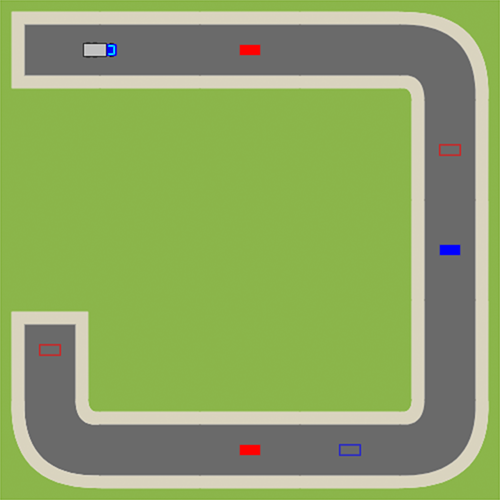
\includegraphics[width=\textwidth]{gfx/exercises-world-d.png}
%     \caption{Beispiel einer Mikrowelt}
%   \end{subfigure}\hfill
%   \begin{subfigure}[b]{0.30\textwidth}
%     \includegraphics[width=\textwidth]{gfx/exercises-program-5.png}
%     \caption{Beispiel eines Programms, welches die Welt löst}
%   \end{subfigure}\hfill
%   \caption{Beispiel Mikrowelt und Minisprache}
% \end{figure}

%************************************************
% Grundlagen
%************************************************
\chapter{Grundlagen}
\label{sec:basics}

In diesem Kapitel werden einige Grundlagen vermittelt, auf welche in späteren Teilen dieser Arbeit verwiesen wird. Aus den Abschnitten "\nameref{sec:basics:playful-learning}" und "\nameref{sec:basics:mini-languages}" werden zudem Anforderungen an diese Arbeit abgeleitet.

%************************************************
% Spielerisches Lernen
%************************************************
\section{Spielerisches Lernen}
\label{sec:basics:playful-learning}

Die im Rahmen dieser Arbeit entwickelte Software soll Lehrer dabei unterstützen, ihren Schülern die Grundlagen des Programmierens zu vermitteln. Dies soll spielerisch geschehen. Prensky führt in seinem Buch \textit{Digital Game-Based Learning} drei Gründe an, warum digitales spielerisches Lernen funktioniert~\cite[147]{prensky2007}:

\begin{enumerate}
    \item Der erste Grund ist das zusätzliche Engagement, das dadurch entsteht, dass das Lernen in einen Spielkontext gebracht wird. Dies kann beträchtlich sein, besonders wenn Menschen nicht lernen wollen.
    \item Der zweite Grund ist der interaktive Lernprozess. Dieser kann und sollte abhängig von den Lernzielen viele verschiedene Formen annehmen.
    \item Der dritte Grund ist die Art und Weise, wie die zwei ersten Gründe im Gesamtpaket zusammengefügt werden. Es gibt viele Möglichkeiten, dies zu tun, und die beste Lösung ist sehr kontextabhängig.
\end{enumerate}

Des Weiteren hängt der Lernerfolg auch immer stark davon ab, wie Spiele vom Lehrer letztendlich eingesetzt werden, aber auch der Stil des Spieles spielt eine Rolle. Damit Spiele -- Lehrspiele im speziellen -- Spaß bringen, müssen sie einige Anforderungen erfüllen. Malone stellt in seinem Artikel \textit{What Makes Computer Games Fun?} eine Checkliste auf, die sich in drei Kategorien gliedert und unter anderem die folgenden Fragen enthält~\cite[49]{malone1981}:

\begin{itemize}
    \item \emph{Herausforderung}: Hat das Spiel ein Ziel? Hat das Spiel einen variablen Schwierigkeitsgrad? Verfügt die Aktivität über mehrere Ziele, z.~B. Zählen von Punkten oder schnelle Reaktionen? Enthält das Programm Zufall? Enthält das Programm versteckte Informationen, die selektiv aufgedeckt werden?
    \item \emph{Fantasie}: Enthält das Programm eine emotional ansprechende Fantasie? Hängt die Fantasie instinktiv mit der in der Aktivität erlernten Fähigkeit zusammen? Ist die Fantasie eine nützliche Metapher?
    \item \emph{Neugierde}: Gibt es audio- und visuelle Effekte, um die Neugier der Sinne zu stimulieren? Gibt es Elemente, die die kognitive Neugier wie Überraschungen oder konstruktives Feedback stimulieren?
\end{itemize}

Diese Anforderungen sollten bei der Aufstellung der Anforderungen für das im Rahmen dieser Arbeit entwickelte Programm berücksichtigt werden, auch wenn sich aufgrund der für diese Art von Lernspiel notwendigen, im nächsten Abschnitt beschriebenen Mechaniken, nicht alle aufgestellten Anforderungen erfüllen lassen werden.

%************************************************
% Minisprachen
%************************************************
\section{Minisprachen}
\label{sec:basics:mini-languages}

Minisprachen sind Programmiersprachen, die speziell auf die Anforderungen von Programmieranfängern zugeschnitten sind, indem sie einen reduzierten Sprachumfang bieten, der speziell auf die Lösung einer bestimmten Klasse von Problemstellungen zugeschnitten ist und dabei die Grundprinzipien des Programmierens hervorhebt bzw. deren Erlernen fördert.

Warum das Erlernen von Programmierfähigkeiten mithilfe von Minisprachen im Gegensatz zu den breit genutzten Universalsprachen (wie z.~B. Java oder C) sinnvoll ist, erklären Brusilovsky et al., indem sie drei Probleme von Universalsprachen für die Anwendung zum Lernen nennen, die Minisprachen zu beheben versuchen \cite[67]{brusilovsky1997}:

\begin{itemize}
    \item Universalsprachen sind zu groß und zu idiosynkratisch. Die konzeptionelle Basis der Sprache bildet zusammen mit den Hauptprinzipien der Programmierung eine große Menge an Material. Anstatt die Grundprinzipien hervorzuheben, rufen die Sprachen nebensächlich Begriffe auf, die die Feinheiten der jeweiligen Sprache und deren Umsetzung, nicht aber die Hauptprinzipien der Programmierung widerspiegeln.
    \item Universalsprachen fördern nicht das Verständnis ihrer grundlegenden Aktionen und Kontrollstrukturen. Die Sprachen sind nicht visuell und ihre Grundfunktionen werden hinter einer undurchsichtigen Barriere ausgeführt. Wenn der Prozess der Programmausführung verborgen ist, entwickelt der Student ein Input-Output-orientiertes Verständnis. Auf diese Weise behindert das Fehlen von visuellem Feedback die Beherrschung der Sprachsemantik.
    \item Da sich Universalsprachen an der Zahlen- und Symbolverarbeitung orientieren, sind die ersten möglichen Aufgaben, die beim Unterrichten der Sprache umgesetzt werden können, weit von den Alltagserfahrungen der Schüler entfernt. Die Entwicklung von Anwendungen, die sowohl informativ als auch interessant sind, erfordert das Erlernen einer beträchtlichen Untermenge der Sprache und das Schreiben recht großer Programme.
\end{itemize}

Brusilovsky et al. heben in Ihrem Artikel \textit{Mini-languages: a way to learn programming principles} einige sich daraus ergebende Eigenschaften von Minisprachen als besonders wichtig hervor \cite[73-74]{brusilovsky1997}:

\begin{itemize}
    \item Sowohl Syntax, als auch Semantik der Sprache sollten \emph{einfach} sein.
    \item Die Operationen der Minisprache sollten \emph{sichtbar} sein. Die meisten Operationen, die der Akteur ausführt, sollten sichtbare Änderungen in der auf dem Bildschirm dargestellten Mikrowelt \TODO{erklären?} vornehmen.
    \item Die Minisprache sollte für die vorgesehene Kategorie von Studenten \emph{attraktiv} und aussagekräftig sein.
    \item Die Sprache sollte \emph{dialogorientiert} sein. Das bedeutet, dass die Sprache Befehl für Befehl in einem Navigationsmodus ausgeführt werden kann (Einzelbefehlsausführung) und als Ganzes in einem Programmiermodus (komplexe Programmausführung).
    \item Die Sprache sollte \emph{modular} sein. Sie sollte einen Mechanismus zum Erstellen abstrakter Anweisungen (Prozeduren) enthalten. Alle Verfahren sollten unabhängige Einheiten sein. Eine solche Prozedur kann als neuer Befehl des Akteurs betrachtet werden, der sowohl im Navigations- als auch im Programmiermodus verwendet werden kann.
\end{itemize}

Aus der Liste dieser Anforderungen ergeben sich direkte Anforderungen an die für diese Arbeit entwickelte Minisprache (siehe \ref{sec:requirements:program}). Sie sind auch -- soweit das beurteilt werden kann -- in allen im nächsten Kapitel genannten vergleichbaren Arbeiten berücksichtigt.

%! Author = Yannick Schröder
%! Date = 17.08.20

%************************************************
% Anforderungsanalyse
%************************************************
\chapter{Anforderungsanalyse}
\label{sec:requirements}

Ziel dieser Arbeit ist die Evaluierung und Migration von GraphQL in die von Marcus Riemer entwickelte Lehr-Entwicklungsumgebung BlattWerkzeug zur Verbesserung des aktuell genutzten Systems.
Nachfolgend wird in diesem Kapitel die Funktionsweise des aktuellen Systems. 
Anschließend werden Anforderungen formuliert und evaluiert die ein neues System größtenteils erfüllen muss.

\section{Aktuelles System}
\label{sec:requirements:system}

Marcus Riemer hat im Rahmen seiner Master-Thesis an der Fachhochschule Wedel die Lehr-Entwicklungsumgebung BlattWerkzeug als Webapplikation entwickelt,
die sich an Kinder und Jugendliche richtet. Mit BlattWerkzeug lassen sich, gestützt durch Drag \& Drop-Edi\-toren,
für beliebige SQLite-Datenbanken Abfragen formulieren und Oberflächen entwickeln~\cite[2]{riemer2016}.
Seit dem Abschluss der Master-Thesis wird BlattWerkzeug im Rahmen eines Promotionsvorhabens weiterentwickelt.

%Server:
Der Server dieser Web-App ist auf Basis von Ruby on Rails gebaut. Er dient hauptsächlich der Speicherung und Auslieferung von Daten.
Kommuniziert wird über eine REST-artige JSON-Schnittstelle~\cite[94]{riemer2016}.

%Client:
Der Client wurde als eine Single-Page Application mit rein clientseitiger Visualisierung aufgebaut,
die lediglich für den Zugriff auf serverseitige Resourcen  (Datenbank, gespeicherte Ressourcen, gerenderte Seiten) Roundtrips zum Server nutzt~\cite[94-95]{riemer2016}.
Programmiert wurde sie 2016~\cite[1]{riemer2016} auf Basis von Angular 2 in TypeScript.
Zum aktuellen Zeitpunkt wird allerdings auf die Angular Version 9.1.0 gesetzt.

%Datenbanksystem
Für die Wahl des einzusetzenden Datenbanksystems wurde sich beim Entwicklungsstart, auf Grund der Kriterien "Kostenlose Verfügbarkeit",
"Einfacher Betrieb", "Einfache Backups", "Tools zur Modellierung" und "Externe Tools zur Entwicklung von SQL-Abfragen"
für eine SQLite Datenbank entschieden~\cite[99-100]{riemer2016}. Im November 2017 ist dann der Grundstein gelegt worden,
um den Server mit einer PostgreSQL Datenbank zu verbinden~\cite{riemerPostgresCommit}, da diese es unter anderem ermöglicht JSON Objekte direkt zu speichern,
ohne diese in Text Datentypen konvertieren zu müssen.

Anhand eines Praxisbeispiels wird im Weiteren die Funktionsweise des Systems in Hinblick auf das Hinzufügen neuer Daten
unter Gewährleistung der Typsicherheit (siehe Unterabschnitt~\fullref{req:typesafe}) verdeutlicht.

\section{Praxisbeispiel - Erweiterung des Datenkonstruktes}
\label{sec:requirements:example}

Damit neue Datensätzen zwischen Server und Client typsicher ausgetauscht werden können sind mehrere Schritte erforderlich.
Die Reihenfolge der nachfolgend aufgeführten Schritte ergibt sich aus dem bisherigen Entwicklungsprozess.

\subsection{Anlegen des Typescript Interfaces}
\label{sec:requirements:example:interface}

Als erstes wird ein Typescript Interface für den Datensatz erstellt, der abgebildet werden soll.
Wir erweitern den Datentyp \emph{Project} aus Listing~\ref{fig:basics:graphql:3} erneut:

\begin{lstlisting}[language=JavaScript,float=h!,caption={Typescript Interface für die Darstellung eines Projektes}, label={lst:example:projectdesc}]
export interface Project {
    id: string;
    name:object;
    public?: boolean;
    slug?: string;
    userId?: string;
    createdAt?: string;
    updatedAt?: string;
}
\end{lstlisting}

\begin{itemize}
    \setlength\itemsep{-1em}
    \item \emph{id/public}: siehe Listing~\ref{fig:basics:graphql:3}.
    \item \emph{name}: hat sich zu einem multilingualen Feld geändert. object repräsentiert den nicht Primitiven Datentyp, also alles was nicht number, string, boolean, symbol, null oder undefined ist~\cite{typescript-object}.
    \item \emph{slug}: ist ein aus einem oder wenigen Wörtern bestehender benutzer- und suchmaschinenfreundlicher
    Text (sprechender Name) als Bestandteil einer URL~\cite{slug-wikipedia}. Diese Angabe ist optional.
    \item \emph{userId}: ist die ID des Nutzers dem dieses \emph{Project} zugeordnet ist (Fremdschlüsselbeziehung).
    \item \emph{createdAt}: ist die optionale zeitliche Angabe wann dieses \emph{Project} erstellt wurde.
    \item \emph{updatedAt}: ist die optionale zeitliche Angabe wann dieses \emph{Project} zuletzt verändert wurde.
\end{itemize}

Wird dieser Datensatz beim Server angefragt, lässt sich die Antwort des Servers auf eine Variable mit dem Typ \emph{Project} zuweisen.
Dadurch wird zur Kompilierzeit ermöglicht typsicher auf die einzelnen Felder des Interfaces zugreifen zu können.

Im nächsten Schritt wird das Interface dem Server zur Verfügung gestellt.

%List Interface/Response Interface
%Dokument Interface
\subsection{Generierung der JSON Schema Definitionen}
\label{sec:requirements:example:schema}
Das Interface aus Listing~\ref{lst:example:projectdesc} wurde clientseitig erstellt und kann auch nur dort verwendet werden. Um es serverseitig nutzen zu können wird daraus eine JSON Schema Datei generiert.
Für die Generierung sind Einträge in einem Makefile nötig, welches sich um die Erstellung aller JSON Schema Dateien, kümmert. Nach der Generierung befinden sich zu jedem aufgeführten Typescript Interface ein passendes JSON Schema in einer eigenen Datei. Diese werden dann in einem Schema Ordner auf Projekt Ebene gehalten. Das jedes Schema in einer eigenen Datei gespeichert ist, kommt dem Server bei der Validierung zu gute. 
Dieser Lädt die Datei, dessen Namen äquivalent zum ursprünglichen Typescript Interface ist, aus dem Ordner, liest das Schema aus und kann dieses zu Validierungszwecken nutzen.

\begin{lstlisting}[float=h!,caption={TypeScript Interface für die Project Darstellung in einer Liste}, label={lst:example:makefile}]
Project.json : $(SRC_PATH)/shared/project.ts
$(CONVERT_COMMAND)
\end{lstlisting}

Mithilfe der JSON Schema Dateien können dann Datensätze validiert werden.

\subsection{Anlegen des Models in Rails}
\label{sec:requirements:example:model}

Sollte das Interface aus Listing~\ref{lst:example:projectdesc} einer neuen Datenbanktabelle entsprechen, muss eine Active Record Migration erstellt werden,
die das Datenbankschema erweitert~\cite{rails-migration}.

\begin{lstlisting}[language=Ruby,float=h!,caption={Rails Migration zum hinzufügen einer \emph{projects} Datenbanktabelle}, label={lst:example:migration}]
create_table "projects", id: :uuid, do |t|
	t.string "slug"
	t.hstore "name", default: {}, null: false
	t.uuid "user_id"
	t.datetime "created_at", null: false
	t.datetime "updated_at", null: false
end
\end{lstlisting}

Durch Ausführung der Migration aus Listing~\ref{lst:example:migration} wird eine neue Tabelle mit der Bezeichnung \emph{projects} erstellt.
Hinzukommend wird ein Active Record Model benötigt, dem die \emph{projects}-Tabelle zugeordnet wird.
Zur Realisierung wird eine Ruby Klasse, die
von der Klasse ApplicationRecord erbt, mit dem selben Namen den die Tabelle hat erstellt.
Die Rails Konvention sieht vor das Datenbanktabellen im Plural und das dazugehörige Model im Singular benannt wird~\cite{rails-naming-convention}.

\begin{lstlisting}[language=Ruby,float=h!,caption={Model}, label={lst:example:model}]
class Project < ApplicationRecord
	# The owner if this project
	belongs_to :user
end
\end{lstlisting}

Auf diese Weise entsteht die Möglichkeit, die Spalten jeder Zeile in dieser Tabelle mit den Attributen der Instanzen des Models abzubilden.
Jede Zeile dieser Tabelle stellt also ein "Projekt" Datensatz mit den in Listing \fullref{sec:requirements:example:interface} aufgeführten Feldern dar.

Um nun auf Anfragen reagieren und Daten aus Model Instanzen an den Client liefern zu können bedarf es einem Controller.

\subsection{Anlegen eines Controllers in Rails}
\label{sec:requirements:example:controller}
Controller haben die Aufgabe Anfragen zu verarbeiten, die vom Router (siehe Listing~\ref{lst:example:router}) an sie weitergeleitet wurden.
Die Funktionen innerhalb eines Controllers sind dafür verantwortlich den Anfragen einen "Sinn" zu geben und die entsprechende Antwort zu erzeugen.
Bei einer Anfrage die Projekt-Daten ausgeliefert bekommen soll, kümmert die Controller Funktion sich darum alle Daten aus dem \emph{Project}-Model
zu holen und gibt diese dann wie bei REST APIs üblich in JSON Form zurück.

\begin{lstlisting}[language=Ruby,float=h!,caption={Route entspricht URL '/project/' und leitet Anfrage an die ProjectsController Funktion \emph{index} weiter }, label={lst:example:router}]
scope 'project' do
	get '/', controller: 'projects', action: :index
end
\end{lstlisting}

\begin{lstlisting}[language=Ruby,float=h!,caption={Controller mit Funktion zum zurückgeben aller Project Instanzen}, label={lst:example:controller}]
class ProjectsController < ApplicationController
	def index
		render json: Project.all
	end
end
\end{lstlisting}

In Zeile 3 des Controllers in Listing~\ref{lst:example:controller} werden um das Beispiel simpel alle Projekte aus der Datenbank geladen und in JSON Form
zurück gegeben. Im aktuellen System hingegen werden die Projekte paginiert an den Client geliefert, damit nicht aus Versehen riesige Datensätze an den Client übertragen werden. Um gewährleisten zu können, das die Antwort vom Server auch die erwarteten Daten liefert, wird ein
Test geschrieben der prüft, ob die Antwort dem clientseitig erstellten Interface aus Listing~\ref{lst:example:projectdesc} entspricht.
Für die Validierung wird ein für Ruby entwickelter JSON Schema Validator genutzt.

\begin{lstlisting}[language=Ruby,float=h!,caption={Test überprüft, ob bei Anfrage der Route '/project/' eine Antwort vom Typ Project folgt}, label={lst:example:controller-test}]
it 'lists a single project' do
	FactoryBot.create(:project, :public)
	get "/project/"
	
	expect(response).to have_http_status(200)

	parsed = JSON.parse(response.body)
	expect(parsed['data'].length).to eq 1

	# Validierung gegen  das "Project" interface
	expect(parsed['data'][0]).to validate_against "Project"
end
\end{lstlisting}


\begin{itemize}
	\setlength\itemsep{-1em}
	\item \emph{Zeile 2}: Erstellt eine \emph{Project} Instanz und speichert diese in der Datenbank.
	\item \emph{Zeile 3}: Ein GET Request wird an die Route "/project/" geschickt.
	\item \emph{Zeile 5}: Es wird der HTTP Status 200 erwartet. 
	\item \emph{Zeile 7}: Parst den response body in JSON.
	\item \emph{Zeile 8}: Erwartet das die Länge der empfangenen Datensätze 1 ist.
	\item \emph{Zeile 11}: Validiert die Antwort gegen das JSON Schema \emph{Project}.
\end{itemize}

Der Server hat nun die Fähigkeit auf eine Anfrage nach allen Projekten zu reagieren.
Somit muss der Client noch die Möglichkeit erhalten eine Anfrage zu erstellen und die Antwort grafisch abbilden zu können.

%Für jede Sicht (z.B. Admin/Frontend) eine Route und Controller Funktion.
\subsection{Dataservices auf dem Client}
\label{sec:requirements:example:service}
In der Welt von Angular gibt es eine strikte Trennung zwischen Darstellung und Verarbeitung von Daten~\cite{angular-service}.
Für die Verarbeitung von Daten, wie das Abrufen, werden Angular Services genutzt. Diese sind typischerweise Typescript Klassen,
deren Verwendungszwecke genau definiert sind. Der im Folgenden beschriebene Service hat die Aufgabe Projekt-Daten zu verarbeiten.

\begin{lstlisting}[language=JavaScript,float=h!,caption={Funktion zum Abruf aller Projekte vom Server}, label={lst:example:service}]
@Injectable()
export class ProjectsDataService {
    constructor(private http: HttpClient) { }
    // Die Antwort soll dem Typparameter "Project" entsprechen
    readonly projects = this.http.get<Project>('/project/');
}
\end{lstlisting}

\begin{itemize}
    \setlength\itemsep{-1em}
    \item \emph{Zeile 1}: \emph{@Injectable} stellt sicher, dass der Compiler die notwendigen Metadaten erzeugt, um die Abhängigkeiten der Klasse zu erstellen, wenn die Klasse injiziert wird.
    \item \emph{Zeile 2}: Deklarierung der Klasse/des Services ProjectsDataService
    \item \emph{Zeile 3}: Injizierung des HttpClient~\cite{angular-http} in den Service
    \item \emph{Zeile 5}: Nutzung des HttpClient zur Erstellung eines typisierten HTTP-Requests, welcher zur bereits hinzugefügten Route in Listing~\ref{lst:example:router} führt.
    Dieser wird auf die readonly Variable projects geschrieben.
\end{itemize}

Hinzuzufügen ist, das dieses Beispiel nur bedingt dem aktuellen System entspricht, da im eigentlich eine einheitliche Service Klasse mit einem Cache verwendet wird, von der der ProjectsDataService erbt. Das Aufzeigen der einheitlichen Service Klasse würde jedoch den Rahmen sprengen.

Die Angabe des Antworttyps \emph{Project} in Zeile 5 fungiert dabei zur Kompilierungszeit als Type Assertion~\cite{typescript-typeassertion}
und erleichtert den Zugriff auf die Attribute der Antwort. Der TypeScript Compiler führt während der Laufzeit jedoch keine Überprüfung durch.
Er geht an dieser Stelle davon aus, das der Entwickler spezielle Prüfungen, wie z.B. der Test in Listing~\ref{lst:example:controller-test}, durchgeführt hat.

Die Dartsellung der erhaltenen Daten übernehmen dann Angular Komponenten, in die Services "injiziert" werden können.
Dadurch können Komponenten die Funktionen eines injizierten Services nach Belieben nutzen.

\subsection{Komponenten auf dem Client}
\label{sec:requirements:example:component}

Eine Angular Komponente entspricht einem Teilbaum des DOM-Baums, auch View genannt.
Somit wird eine Komponente für einen bestimmten Zweck erstellt,
der in unserem Fall die grafische Auflistung der Projekt-Daten ist.

\begin{lstlisting}[language=JavaScript,float=h!,caption={Funktion zum Abruf aller Projekte vom Server}, label={lst:example:component}]
@Component({
    selector: "project-list",
    templateUrl: "templates/project-list.html",
})
export class ProjectListComponent {
    // Injizierung des ProjectsDataService
    constructor(private _projectsData: ProjectsDataService) {}

    readonly projects = this._projectsData.projects;
}
\end{lstlisting}

\begin{itemize}
    \setlength\itemsep{-1em}
    \item \emph{Zeile 1}: Annotierung einer Typescript-Klasse als Komponente.
    \item \emph{Zeile 2}: Der Wert von \emph{selector} kann als HTML-Tag (<project-list></project-list>) in Templates genutzt werden,
    um diese Komponente Instanziieren und das zugehörige Template innerhalb des Bezeichners rendern zu können.
    \item \emph{Zeile 3}: Festlegung des Pfades, wo sich das zu rendernde Template, also der darzustellende HTML Code befindet.
    \item \emph{Zeile 5}: Deklarierung der Klasse/des Komponente ProjectListComponent.
    \item \emph{Zeile 7}: Injizierung des ProjectsDataService~\cite{angular-http} in die Komponente.
    \item \emph{Zeile 9}: Speichern der Funktion aus dem ProjectsDataService zum Abrufen der Projekt-Daten auf eine Instanzvariable.
\end{itemize}

Eine Komponente stellt HTML Code dar, der in einer Datei gespeichert wird, die als Template bezeichnet wird.
Innerhalb des Templates ist der Zugriff auf die nicht privaten Variablen der Komponenten gegeben.
Das zugehörige Template project-list.html sieht folgendermaßen aus:

\begin{lstlisting}[language=JavaScript,float=h!,caption={Funktion zum Abruf aller Projekte vom Server}, label={lst:example:service}]
<project-list-item
  *ngFor="let project of projects | async"
  [project]="project"
></project-list-item>
\end{lstlisting}

\begin{itemize}
    \setlength\itemsep{-1em}
    \item \emph{Zeile 1}: Aufruf der Komponente mit dem \emph{selector} "project-list-item".
    Diese übernimmt hier die Darstellung eines einzelnen Projektes innerhalb einer Liste und verdeutlicht damit
    die Modularität von Angular Komponenten.
    \item \emph{Zeile 2}: *ngFor ist die "Repeater"-Direktive ~\cite{ng-for} in Angular.
    Sie ermöglicht ein gegebenes HTML Template einmal für jeden Wert in einem Array zu wiederholen,
    wobei jedes Mal der Array-Wert als Kontext übergeben wird. Das Array \emph{projects} kommt aus der Komponenten in Listing~\ref{lst:example:component} Zeile 9.
    \item \emph{Zeile 3}: Übergibt den Wert aus dem Array an eine mit \emph{@Input()} annotierte Variable \emph{project} aus der "project-list-item" Komponenten.
\end{itemize}

Diese Schritte sind in ihrer Gänze nur bei der Einführung neuer Entitäten notwendig.
Bei der Nutzung von Subtypen kann ein Teil der umgesetzten Schritte wiederverwendet werden,
bzw ist nur einmal erforderlich gewesen, wie das Ausführen einer Datenbankmigration.

\subsection{Anlegen einer neuen Sicht}
\label{sec:requirements:example:newview}

Für das Bereitstellen einer neuen Sicht auf die Projekt Daten sind mehrere Schritte zu wiederholen (siehe Tabelle~\ref{tbl:newview}).

\begin{table}[h!]
    \begin{tabular}{|p{0.12\textwidth}|p{0.52\textwidth}|p{0.12\textwidth}|}
        \hline
        \textbf{Schritt} & \textbf{Beschreibung} & \textbf{Aktuelles \newline System} \\ \hline
        $\ref{sec:requirements:example:interface}$ & Anlegen eines Interfaces & $\surd$  \\ \hline
        $\ref{sec:requirements:example:schema}$ & Eintrag in Makefile & $\surd$\\ \hline
        \multirow{2}{*}{$\ref{sec:requirements:example:model}$}
        & Anlegen einer Datenbank Migration & $X$  \\
        & Anlegen des Models & $X$ \\ \hline
        \multirow{4}{*}{$\ref{sec:requirements:example:controller}$}
        & Route definieren & $\surd$  \\
        & Anlegen des Controllers & $X$  \\
        & Controller Funktion schreiben & $\surd$  \\
        & Tests schreiben & $\surd$  \\ \hline
        \multirow{2}{*}{$\ref{sec:requirements:example:service}$}
        & Anlegen eines Angular Services & $X$  \\
        & Funktion zum Abschicken einer Query & $\surd$  \\ \hline
        \multirow{2}{*}{$\ref{sec:requirements:example:component}$}
        & Anlegen einer Angular Komponenten & $\surd$  \\
        & Anlegen eines Templates & $\surd$  \\ \hline
    \end{tabular}
    \vspace{5pt}
    \centering
    \caption{Vergleich der Funktionweise des aktuellen Systems mit GraphQL in Bezug auf die Erstellung neuer Sichten auf bereits vorhandene Datensätze}
    \label{tbl:newview}
\end{table}

Auffallend ist, dass im aktuellen System 8 von 12 Schritte erneut ausgeführt werden müssen.

\section{Vorteile des bisherigen Ansatzes}
\label{sec:requirements:pros}
Die Verwendung des derzeitigen Systems hat viele Vorteile,
deren Gewichtung in Hinsicht auf die Migration eines neuen Systems zu evaluieren gilt.
Nachfolgend werden die wichtigen Vorteile erläutert.

\subsection{Typescript Typsystem}
\label{sec:requirements:pros:typescript}
Ein Vorteil ist die Verwendung des umfangreichen Typescript Typsystems.
Dieses ermöglicht neben Typüberprüfungen zur Kompilierzeit auch Vererbungen zwischen Interfaces, die Abbildung verschiedenster Typvarianten wie
Union Types, zur ermöglichung verschiedener Typen innerhalb einer Variablen, Intersection Types zum zusammenfügen von Typen,
Generische Typen, sowie Utility Types um bestehende Typen zu manipulieren.
In Abschnitt~\fullref{sec:basics:typescript} wurden bereits mehrere Möglichkeiten dazu vorgestellt.

\subsection{Typescript zu JSON Schema Generatoren}
\label{sec:requirements:pros:generation}
Hinzukommend können "Typescript zu JSON Schema Generatoren" Annotationen innerhalb der Typescript Interfaces verarbeiten~\cite{json-schema-generator-annotations}.
Dadurch können Wertebereiche vorgegeben bzw. eingeschränkt werden,
wie das Setzen eines Minimums bzw. Maximums bei Zahlen, die Verwendung von Reguläre Ausdrücke für Zeichenketten,
die Angabe wie viele Elemente ein Array minimal bzw. maximal aufnehmen kann,
so wie die Angabe wieviele Attribute ein Objekt minimal bzw. maximal haben darf und welche erwartet werden.
Zudem ermöglichen die Generatoren die Bereitstellung der clientseitig erstellten Typdefinitionen in Form von JSON Schema Dateien.

\subsection{Modularität}
\label{sec:requirements:pros:modul}
Aus Unterabschnitt~\fullref{sec:requirements:pros:generation} ergibt sich eine bessere Modularität.
Der Kern des Systems zur typsicheren Kommunikation besteht aus den drei Punkten Typescript Interface, Typescript zu JSON Schema Generator und
JSON Schema Validator. Die ersten beiden Punkte sind unabhängig vom Backend.
Zudem sind JSON Schema Validatoren in 19 Sprachen~\cite{json-schema-implementations} bereitgestellt worden, wodurch das Backend austauschbar ist.
Daher kann der Client auch mit anderen APIs typsicher kommunizieren, wenn diese Zugriff auf dessen Typdefinitionen erhalten.

\subsection{Typsicherheit zur Kompilierzeit}
\label{sec:requirements:pros:typesafe-compile}
Im Client sorgt das Typescript Typsystem durch für Typsicherheit zur Kompilierzeit.

Typsicherheit auf dem Server stellt sich schwieriger dar. In der Welt von Ruby wird nur mit Objekten ohne Typangabe gearbeitet.
Auf eine Variable in der eine Zeichenkette steckt, kann z.B. eine Zahl zugewiesen werden. Wenn anschließend eine Funktion der String Klasse
im guten Glauben das es sich bei der Variablen noch um eine Zeichenkette handelt, auf einer Zahl aufgerufen wird, kommt es zu einem Laufzeitfehler.
Ein ausreichendes Sicherheitsgefühl wurde dennoch durch umfangreiches Testen der Controller, Models und Helper erlangt.

Ungeachtet dessen besteht das Problem, dass zur Laufzeit eingehende Daten ungewollte Beschaffenheiten aufweisen können.

\subsection{Typsicherheit zur Laufzeit}
\label{sec:requirements:pros:typesafe-runtime}
Beim Kompilieren von Typescript zu Javascript werden alle Typinformationen entfernt.
Wenn also Daten von einer Schnittstelle abgerufen werden, kann nicht sichergestellt werden das diese korrekt ankommen, woraus
ungewolltes Verhalten resultieren kann.

Um ungewolltem Verhalten vorzubeugen wurden Fehlerbehandlungen hinzugefügt, bei denen jede Anfrage auf Korrektheit geprüft wird.
Voraussetzung ist, dass eigehende Anfragen gegen den selben Typen validiert werden,
den der Client für das Abschicken nutzt und dieser Typ bei Anfragen zum Erstellen oder Ändern von Daten kompatibel mit dem Datenbankschema ist.
Hinzuzufügen ist das wie in Abschnitt~\ref{sec:requirements:example:schema} beschrieben, aus Interfaces JSON Schema Dateien erzeugt werden,
die für die Validierung vom JSON Schemer Validator gebraucht werden. Somit wird indirekt gegen die Typescript Interfaces validiert.

Zusätzlich wurden auf dem Server Request Specs genutzt.
Diese können zur Kompilierzeit Laufzeitfehler in der API Kommunikation bestmöglich ausschließen.
Sie Testen das Verhalten der Controller, durch abschicken von HTTP-Requests und prüfen, ob die Antwort die erwartete Beschaffenheit ausweist. 

Diese Tests wurden in den Deployment Prozess der Webapplikation eingebaut. Bei fehlgeschlagen einiger Tests wird die Bereitstellung der Software
verhindert, wodurch zur Laufzeit ein typsicheres Verhalten suggeriert wird.

\begin{figure}[h!]
    \centering
    \includegraphics[width=\linewidth]{snippets/server-client-api.pdf}
    \caption{Typsichere Kommunikation zwischen Typescript Client und Ruby Server}
    \label{req:typesafe:server-client-short}
\end{figure}

\subsection{Stabilität}
\label{sec:requirements:pros:stable}
Die Software Blattwerkzeug ist seit mehreren Jahren in der Entwicklung. Von Beginn an (2016) wird
eine REST-artige JSON-Schnittstelle verwendet (siehe Kapitel 4.1. Client-Server-Architektur ~\cite{riemer2016}).
Im laufe der Zeit wurden viele Tests entwickelt die sicher stellen das alles wie erwartet funktioniert.
Somit hat sich das aktuelle System seit mehreren Jahren bewährt.

\section{Nachteile des bisherigen Ansatzes}
\label{sec:requirements:cons:typescript}
Auch wenn ein System funktionstüchtig ist, ist es nicht zwangsläufig perfekt.
In diesem Abschnitt werden die relevanten Nachteile der bisherigen Umsetzung ausgearbeitet.

\subsection{Manuelle SQL Queries}
Für alle im Client darzustellenden Models müssen die zwei Funktionen \lstinline|to_full_api_response| und \lstinline|to_list_api_response| entwickelt werden.
\lstinline|to_full_api_response| selektiert alle Attribute die ein Admin sehen darf. Nur ein Teil dieser Attribute wird im Admin Bereich auch wirklich gebraucht, sie sollen trotzdem dem Admin zugängig gemacht werden.
\lstinline|to_list_api_response| selektiert nur die Attribute die ein normaler Nutzer sehen darf. Dieses Verfahren ist sehr unflexibel und wird schnell aufwendig wenn noch weitere Rollen dazu kommen mit anderen Berechtigungen in Bezug auf das Anzeigen von Daten.
%\subsection{Ruby ohne Typangaben}
%Umfangreiches Testen von untypisiertem Rubycode kann zwar das Gefühl von Sicherheit vermitteln, %dieses hängt allerdings von der Fähigkeit des Programmierers ab, alle möglich Fälle die eintreten %können mit den Tests abzudecken.
%rest-projects-list-huge.png
%Eine alternative Idee dazu wäre die Nutzung eines von vielen Rubygems wie %\emph{typesafe-ruby}~\cite{typesafe-ruby}
%oder \emph{sorbet}~\cite{sorbet} die versprechen Rubycode typsicher zu machen. Diese Tools werden %sich im aktuellen System nicht zu Nutze gemacht.

\subsection{Auswahl von Attributen}
\label{sec:requirements:cons:attributes}
Bei allen im Kontext dieser Arbeit relevanten Listendarstellungen im Client treten Overfetching Probleme auf.
Die Listendarstellung von Projekten im Admin Bereich werden 3 von 11 Attributen in der Liste angezeigt. 
Um dies als Nachteil zu untermauern, wird die Größe des im aktuellen System übertragenen JSON Objektes (siehe Abbildung~\ref{req:rest-projects-list-huge}) mit einem JSON Objekt verglichen, welches nur die 3 anzuzeigenden Attribute der Projektdaten beinhaltet (siehe Abbildung~\ref{req:rest-projects-list-small}). Die Größe eines Objektes ohne überflüssige Attribute, ist bei einer Listengröße von 5 Projekten fast 5 mal kleiner.
Bei den beiden Abbildungen handelt es sich um Screenshots aus dem Firefox Netzwerkanalyse Tool.

\begin{figure}[h!]
	\centering
	\includegraphics[width=\linewidth]{snippets/rest-projects-list-small.png}
	\caption{Anfrage der Projekt Liste und Antwort mit nur den 3 anzuzeigenden Attributen}
	\label{req:rest-projects-list-small}
\end{figure}

\begin{figure}[h!]
	\centering
	\includegraphics[width=\linewidth]{snippets/rest-projects-list-huge.png}
	\caption{Anfrage der Projekt Liste und Antwort mit allen Attributen}
	\label{req:rest-projects-list-huge}
\end{figure}

Möchte man zusätzlich noch Beziehungen abbilden kann ebenfalls das in Abschnitt~\fullref{sec:basics:restapi:interface} beschriebene Underfetching Problem auftauchen.
Dieses ließe sich im aktuellen System durch manuelle Erstellung der SQL Queries beheben.

\subsection{Camel Case und Snake Case Notationen}
Da in Ruby für Benennungen von Variablen, Methoden, Dateien etc. Snake Case und auf dem Typescript Client Camel Case verwendet wird, müssen Datensätze nach auslesen aus der Datenbank vor dem Ausliefern an den Client zu Camel Case konvertiert werden. Das gleiche gilt wenn Anfragen zum Erstellen von Datensätzen an den Server geschickt werden. Bevor diese in die Datenbank eingefügt werden können, muss die Schreibweise der einzelnen Attribute zu Snake Case verändert werden.

\subsection{Am Rande der Skalierbarkeit}
Die Haltung der zur JSON Schema Generierung benötigten Informationen zu jedem Interface - Pfad der Datei, Name des Interfaces, Name der generierten Zieldatei -
in einem Makefile ist unübersichtlich und deren Eintragung kann leicht vergessen werden. 
Ein weiterer Nachteil und Einschränkung des Entwicklers ist der Programmieraufwand bei der Erstellung neuer Abfragen bzw. neuer Sichten (siehe Tabelle~\ref{sec:requirements:example:newview}).
So wie das System aktuell ist skaliert es noch ausreichend. Je größer allerdings die Anwendung wird, je mehr generierte Typen verwendet werden und je mehr unterschiedliche Sichten gebraucht werden desto schlechter skaliert es.

\section{Anforderungen}
\label{sec:requirements:req}
In diesem Abschnitt sind Kernanforderungen an ein neues System formuliert.
Aus dem Abschnitt~\fullref{sec:requirements:system} konnten sich bereits mehrere dieser Anforderungen ableiten lassen.

\subsection{Darstellungsvielfalt}
\label{sec:requirements:req:view}
Als erste Anforderung wird die Darstellungsvielfalt definiert.
In einer Webapplikation, in der Nutzer verschiedene Rollen zugewiesen bekommen, wodurch sie Berechtigungen erhalten,
werden je nach Rolle unterschiedliche Funktionalitäten und Sichten auf Daten gewährt.

Im aktuellen System wird zwischen den Rollen Admin, Owner und User unterschieden - beschrieben in Kapitel 3.2.6 Rollen und Autorisierung
in der Abschlussarbeit von Tom Hilge~\cite{Abschlussarbeit-Tom-Hilge}.
Die relevanten Berechtigungen der einzelnen Rollen sind in Tabelle~\ref{tbl:req:roles} beschrieben.

\begin{table}[h!]
    \begin{tabular}{|p{0.34\textwidth}|p{0.3\textwidth}|p{0.08\textwidth}|p{0.08\textwidth}|p{0.08\textwidth}|}
        \hline
        \textbf{Berechtigung} & \textbf{Beschreibung} & \textbf{Admin} & \textbf{Owner} & \textbf{User} \\ \hline
        \multirow{3}{*}{Sichten im Frontpage Bereich}
        & Projekt Liste & $\surd$ & $\surd$ & $\surd$\\
        & Projekt Details & $\surd$ & $\surd$ & $\surd$\\
        & Projekt Erstellen & $\surd$ & $\surd$ & $\surd$ \\
        \hline
        \multirow{2}{*}{Sichten im Admin Bereich}
        & Erweiterte Projekt Liste & $\surd$ & $X$ & $X$\\
        & Erweiterte Projekt Details & $\surd$ & $X$ & $X$\\
        \hline
        \multirow{1}{*}{Geplante Sichten}
        & Projekt Liste eines Owners & $\surd$ & $\surd$ & $X$\\
        \hline
    \end{tabular}
    \vspace{5pt}
    \caption{Zugriffsberechtigungen auf Projekt Daten der verschiedenen Rollen zur Hervorhebung der benötigten Darstellungsvielhalt}
    \label{tbl:req:roles}
\end{table}

Viele dieser Sichten nutzen unterschiedliche Subtypen des Projekttypen.
Beispielsweise listet die Projektliste auf der Frontpage nur öffentliche Projekte - bei denen das Attribut \emph{public} auf \emph{true} gesetzt ist -
auf und zeigt dabei die Datenfelder "name", "description", "slug" und "defaultProgrammingLanguage" an.
Die Projektliste im Adminbereich zeigt im Gegensatz dazu alle Projekte an und greift auf
die Datenfelder "name", "slug", "Anzahl der Code Ressourcen" und die "id" zu.
Die Bedeutung der Felder "defaultProgrammingLanguage" und "Anzahl der Code Ressourcen" ist in diesem Kontext irrelevant und wird nicht näher erläutert.

Zu diesen unterschiedlichen Sichten kommen noch Weitere Spezifikationen in der Dartsellung die gefordert sind.

\subsubsection{Mehrsprachigkeit}
Die Webapplikation von Marcus wird aktuell in zwei Sprachen Angeboten, Deutsch und Englisch.
In Abbildung~\fullref{fig:basics:graphql:6} wurde bereits suggeriert das das Feld \emph{name} eines Projektes nach Sprachen gefiltert werden kann.
Bislang wurde \emph{name} als reiner string behandelt (siehe Listing~\ref{lst:example:projectdesc}). Im aktuellen System werden Mehrsprachige Felder
als hstore (Hash mit Tiefe 1) in der Datenbank gehalten. Der Schlüssel gibt den zweistelligen Ländercode nach ISO Alpha-2 \cite{iso-alpha-2} an
und der dazugehörige Wert den Namen des Projektes in der jeweiligen Sprache.

\begin{lstlisting}[language=JavaScript,float=h!,caption={Speicherung der Projektnamen als jsonb}, label={sec:requirements:multilang}]
{
    "de"=>"Drei Fragezeichen",
    "en"=>"Three Investigators"
}
\end{lstlisting}

Das Sprachenangebot gilt bei einer Systemmigration weiterhin als gefordert und soll zukünftig erweiterbar sein.

\subsubsection{Sortieren und Paginierung}
Die Paginierung ist das Portionieren großer Datensätze zur übersichtlicheren und schnelleren Verarbeitung und Darstellung.
In Blattwerkzeug werden alle Listenansichten im Admin Bereich in einer Tabelle paginiert angezeigt.
Ein Datensatz der einer Liste mit 30 Einträgen entspricht würde bei einer Paginierung mit der Seitengröße 5 auf 6 Seiten aufgeteilt werden.
Ein Menü zum traversieren der Einträge könnte wie in Listing~\ref{req:view:pagination} aussehen.

\begin{figure}[h!]
    \centering
    \includegraphics[width=\linewidth]{snippets/paginierung.pdf}
    \caption{Menüleiste zum Wechseln der Seite und Einstellen der Seitengröße}
    \label{req:view:pagination}
\end{figure}

Hinzukommend soll es möglich sein eine Liste nach verschiedenen Attributen sortieren zu können, auch wenn diese mehrsprachig sind und
in der Datenbank als hstore (siehe Abschnitt~\ref{sec:basics:postgres}) gespeichert werden.

\subsubsection{Filtern}

Für Listendarstellungen soll es möglich serverseitig Einträge effizient, also möglichst direkt in SQL zu filtern.


\subsection{Typdefinitionen}

Typdefinitionen (als Ganzes Typschema genannt) sind die Grundlagen für typsichere Webapplikationen.

Gefordert wird, dass sowohl serverseitige, als auch clientseitige Applikationen sich ein Typschema teilen. 
Die Alternative, dass jede Applikation ein eigenes Typschema hält ist keine Option. Diese müssten mit viel Aufwand zu jedem Zeitpunkt synchron gehalten werden, wodurch bei jeder Änderung eines Schemas alle Weiteren angefasst werden müssten. Dies würde keine Verbesserung zum aktuellen System bedeuten.

Somit muss ein Typschema, wie in Listing~\fullref{req:typesafe} erwähnt, systemübergreifend zur Verfügung gestellt werden.

\subsubsection{Übersetzung des Typschema durch Codegenerierung}
Codegeneratoren ermöglichen das Übersetzen eines Typschemas in ein Anderes, wie z.B. von Typescript zu JSON Schema.
Sie sind für die zentrale Haltung und Nutzung nur eines Typschemas ausschlaggebend.

Gefordert ist bei der Einführung eines Typschemas, das entsprechende Generatoren für alle angebundenen Applikationen vorhanden sind.

\subsubsection{Datenbankschema}
Zusätzlich wird gefordert, dass das Typschema mit dem bereits vorhandenen Datenbankschema kompatibel ist.
Bei Abweichungen, wie der Speicherung eines Datums in verschiedenen Datumsformaten,
werden Übersetzungen nach auslesen oder vor dem Einfügen in die Datenbank gefordert.

Codegeneratoren können hierbei nur in eine Richtung genutzt werden.
Diese bezieht sich auf die Generierung von Typen aus dem Datenbankschema zum Beispiel mithilfe des Rubygems \emph{schema2type}~\cite{schema2type}.

Die Generierung eines Datenbankschemas aus Typdefinitionen ist nicht zu empfehlen.
Zum einen muss für jeden Typen angegeben werden, ob dieser eine Datenbanktabelle darstellt oder z.B. nur ein Subtyp ist.
Zum anderen sind komplexe Beziehungen zwischen Typen schwer abzubilden.

Also ist mit einer Koexistenz zwischen zentralem Typschema und Datenbankschema zu rechnen.

\subsubsection{Synchronisation der Typdefinitionen}
Sollte das zentrale Typschema für eine Applikation übersetzt werden,
müssen das übersetzte Schema synchron zum Ursprünglichen bleiben. Dies sollte in den Prozess der Bereitstellung der Software eingebunden werden.

Ein neues System muss also folgende Anforderungen erfüllen:

\begin{itemize}
    \setlength\itemsep{-1em}
    \item Zentrales Typschema
    \item Übersetzung des Typschemas für jede Applikation
    \item Synchronität aller Schemata
    \item Kompatibilität mit Datenbankschema
\end{itemize}

\subsection{Typsicherheit}
\label{req:typesafe}
Eine weitere grundlegende Anforderung bei der Entwicklung einer Webapplikation ist die Typsicherheit.
Im Kontext der Arbeit werden Typsicherheit auf dem Client,
dem Server und die typsichere Kommunikation zwischen Client und Server miteinander in Bezug gebracht.
Sind die drei Punkte gegeben wird von einer Typsicheren Webapplikation gesprochen.

\subsubsection{Auf dem Client und Server}
\label{req:typesafe:client}
Die Typsicherheit ist im aktuellen System clientseitig und serverseitig ausreichend gegeben (siehe Unterabschnitt~\fullref{sec:requirements:pros:typesafe-compile} und Unterabschnitt~\fullref{sec:requirements:pros:typesafe-runtime}).
Es wird mindestens gefordert das sich diese mit Einführung eines neuen Systems nicht verschlechtert.

\subsubsection{Kommunikation zwischen Server und Client}
\label{req:typesafe:api}
Während des Datenaustausches zwischen Client und Server kann es durch fehlerhafte Daten zu Laufzeitfehlern kommen.
%Diese sind in einer Webapplikation sehr unschön, da außer bei einer fehlerhaften Eingabe in Formularen, dem Nutzer
%meist lediglich gezeigt wird das etwas schief gelaufen ist, dieser aber keine Möglichkeit zur Fehlerbehebung erhält.

Dieses Problem lässt sich bei eingehenden Daten durch Validierungen jeder Anfrage und Antwort auf ihre Korrektheit lösen.
Vorausgesetzt ist, dass jede eingehende Anfrage gegen den \textbf{selben} Typen validiert wird,
den der Client auch für das Abschicken nutzt und kompatibel mit dem Datenbankschema ist.
Umgekehrt gilt, dass jede Antwort gegen den selben Typen serverseitig validiert wird, den der Client zur Speicherung der Antwort verwendet.
Voraussetzung dafür sind systemübergreifende Typdefinitionen, in Abbildung~\ref{req:typesafe:server-client-short} SCHEMA genannt.

Die folgenden Beispiele zeigen in welchem Ausmaß die Validierung der Daten gefordert ist. In Abbildung~\ref{req:typesafe:request-validation} wird durch ein Formular die Erstellung eines Projektes demonstriert. Die Inhalte des Formulars werden auf ein Objekt vom Typ \emph{CreateProjekt} (siehe Listing~\ref{req:typesafe:createproject}) geschrieben und an den Server geschickt. Dort wird der eingehende Datensatz gegen den selben Typ validiert. Treten hierbei Fehler auf, wird der Datensatz nicht in die Datenbank geschrieben und der HTTP Status 400 zurück gegeben.
Wird der Datensatz erfolgreich validiert, wird der Datensatz in der Datenbank gespeichert und der HTTP Status 200 an den Client geschickt.

\begin{lstlisting}[language=Javascript,float=h!,caption={Interface zum Erstellen eines Projektes}, label={req:typesafe:createproject}]
interface CreateProject {
  name: string;
  slug?: string;
  public: boolean;
}
\end{lstlisting}

\begin{figure}[h!]
	\centering
	\includegraphics[width=\linewidth]{snippets/project-create-validation.pdf}
	\caption{Validierung von Requests zum Erstellen eines neuen Projekt Datensatzes}
	\label{req:typesafe:request-validation}
\end{figure}

In Abbildung~\ref{req:typesafe:list-validation} wird eine Liste von Projekten deren Attribut \emph{public} auf \emph{true} gesetzt ist beim Server angefragt. Bevor diese Liste an den Client zurück gegeben wird, wird gefordert, dass diese gegen das Interface validiert wird, welches der Client zur Darstellung nutzt (siehe Listing~\ref{req:typesafe:listproject}). Schlägt die Validierung fehl, wird der HTTP Status 400 zurück gegeben, ansonsten der Datensatz (inkl. HTTP Status 200).

\begin{lstlisting}[language=Javascript,float=h!,caption={Interface zum Auflisten von Projekten}, label={req:typesafe:listproject}]
interface ListProject {
  id: string;
  name: string;
  slug?: string;
}
\end{lstlisting}

\begin{figure}[h!]
    \centering
    \includegraphics[width=\linewidth]{snippets/project-list-validation.pdf}
    \caption{Validierung von Responses zum Auflisten von Projekt Datensätzen}
    \label{req:typesafe:list-validation}
\end{figure}

Ein neues System muss als Anforderung mindestens den aktuellen Grad an Sicherheit aufweisen durch:

\begin{itemize}
    \setlength\itemsep{-1em}
    \item Systemübergreifendes Validieren gegen die selben Typen
    \item Validierung von Anfragen
    \item Validierung von Antworten
    \item Testen der Schnittstellen, um Laufzeitfehler vorzubeugen.
\end{itemize}

%Erfordert applikationsübergreifende Typdefinitionen.
%JSON Schema Validator für Datenbankfelder:
%/models/json schema validator
%JSON Schema Validator für Requests:
%grammars controller update
%JSON Schema Validator für Responses:
%Rspec
%JSON Schema Erzeugung aus Typescript Interfaces:
%Aktuell werden Clientseitig JSON Schema Dateien mithilfe von Typescript Interfaces und einem ellenlangen Makefile generiert.

\subsection{Performance und Skalierbarkeit}
Performanz und Skalierbarkeit sind bei der Wahl eines Systems ausschlaggebende Kriterien. Das aktuelle System weist im Bereich der Kommunikation Schwächen auf, die es zu Beheben gilt.

\subsubsection{Over- und Underfetching}
Over- und Underfetching sind für eine REST API typische Probleme.
In Unterabschnitt~\fullref{sec:requirements:cons:attributes} wurde bereits gezeigt weshalb diese ein Nachteil in der Performanz darstellen.
Ein neues System sollte diese Probleme beheben können.
Wichtig ist, dass nicht für jede gekürzte Sicht ein Subtyp und eine neue Route inkl. Controllerfunktion erstellt wird. Des weiteren dürfen Beziehungen zwischen Daten nicht das Abfeuern übermäßig vieler Requests bedeuten.

\subsubsection{N+1 Query Problem}
Ein Weiterer Aspekt der die Performanz und Skalierbarkeit einschränkt ist das N+1 Query Problem bei Datenbankabfragen. Dieses unterscheidet sich kaum zu dem bereits erwähnten N+1 Query Problem bei Abfragen an die Web API. Beide Beschreiben einen Engpass der bei Hochskalierung von Anfragen zu Einbußen in der Performanz führt. 

Datenbankabfragen werden auch nach der Migration eines neuen Server Roundtrip Verfahrens serverseitig von Rails ausgeführt. Wurde das N+1 Query Problem beim Anfrage der Web API gelöst, kann es dennoch zum Abschicken von N+1 Datenbankabfragen kommen.

Dieses Problem gilt als Anforderung zu lösen.

\subsubsection{Cache}
Die Nutzung eines Caches soll bei HTTP Anfragen bereitgestellt werden.
TODO: Weiter ausführen, aber kurz halten


\begin{itemize}
	\setlength\itemsep{-1em}
	\item Lieferung nur benötigter Daten
	\item Abschicken möglichst weniger Anfragen an die Web API
	\item Abschicken möglichst weniger Anfragen an die Datenbank
	\item Möglichkeit zur Nutzung eines Caches
\end{itemize}

\subsection{Validierung von jsonb und hstore}
\label{req:validation:json}
Eine der Sonderanforderungen ist das Validieren von Entitäten aus der Datenbank, die ein JSON Objekt beinhalten.
Manche zum Beispiel Abstrakte Datentypen wie eine Map lassen sich erschwert in ein Datenbankschema gießen. Sie können dann als json,
jsonb oder hstore in ihrer Gesamtheit gespeichert werden, ohne das für Schlüssel und Werte Bedingungen (Constraints) auf Datenbankebene definiert werden können.

Gefordert wird das diese JSON Objekte gegen einen Typen aus dem Typschema validiert werden, bevor sie in die Datenbank eingefügt werden. Sollten die JSON Objekte ebenfalls nicht im Typschema des neues Systems abbildbar sein und dadurch implizit validiert werden können, müssen sie mindestens gegen das bereits existierende JSON Schema validiert werden.

\subsection{Benennungskonvention}
Die Verwendung verschiedener Benennungskonventionen kann problematische Folgen haben.
In der Welt von Ruby werden Woertrennungen in Dateinamne, Variablennamen, sowie Funktionsnamen mit Unterstrichen getrennt (Snake Case).
In Typescript sieht die Konvention vor Variablen- und Funktionsnamen in Camel Case und Klassennamen in Pascal Case zu schreiben~\cite{typescript-conventions}.

Diese Gegebenheit erschwert die Kommunikation zwischen Typescript Client und Ruby Server. Anforderung ist, das ein neues System mit diesen Unterschieden umgehen kann.

%************************************************
% Implementierung
%************************************************
\chapter{Implementierung}
\label{sec:implementation}

In diesem Kapitel wird die Implementierung des im Rahmen dieser Arbeit entwickelten Programms dargestellt, sowie die technischen Entscheidungen, die zu ihr geführt haben, erläutert. Außerdem beschreibt dieses Kapitel die Integration des entstandenen Tools in BlattWerkzeug.

%************************************************
% Rahmenhandlung
%************************************************
\section{Rahmenhandlung}
\label{sec:implementation:story}

Für die Festlegung einer Rahmenhandlung bieten sich im wesentlichen zwei Vorgehensweisen an:

\begin{enumerate}[noitemsep]
  \item Es wird zunächst eine Logik entwickelt und teilweise bereits implementiert. Die Rahmenhandlung wird erst später festgelegt und richtet sich nach den gewünschten und ggf. implementierten Funktionen. Mit dieser Vorgehensweise lässt sich die Logik noch klarer von der Darstellung trennen. Die Darstellung wird austauschbar und es ist sogar denkbar, verschiedene Rahmenhandlungen auf derselben Logik zu implementieren. Ob in der endgültigen Rahmenhandlung nun also Roboter oder Marienkäfer vom Programm gesteuert werden, wird erst definiert, wenn die Struktur der Programme festgelegt wurde.
  \item Eine andere Vorgehensweise ist es, die Rahmenhandlung direkt am Anfang festzulegen. Die Anforderungen der Rahmenhandlung diktieren in diesem Fall die Logik. Naturgemäß fließen Anforderungen an die Logik bei der Festlegung der Rahmenhandlung auch hier mit ein. Allerdings sind Darstellung und Logik bei dieser Vorgehensweise viel enger aneinander geknüpft. Ein späteres Austauschen der Darstellung wird deutlich erschwert. Die engere Verbindung bedeutet allerdings auch eine bessere Abstimmung der beiden Komponenten.
\end{enumerate}

Für diese Arbeit wurde die zweite Vorgehensweise gewählt, um so die Minisprache besser auf die Rahmenhandlung abstimmen zu können, und im ersten Schritt unter Berücksichtigung der Anforderungen an die Logik eine Entscheidung über eine Rahmenhandlung getroffen. Das Ziel ist es, mithilfe eines Lastwagens, welcher vom Spieler über Programmbefehle steuerbar ist (siehe \ref{sec:requirements:program}), über ein Netz von Straßen, verschiedenfarbige Container an ihre vorgesehenen Ablageorte zu bringen. Dabei ist die Ladefläche des Lastwagens auf einen Container begrenzt, womit unter Umständen zur Lösung mehrfache Fahrten -- auch Teilfahrten -- notwendig werden können. Dargestellt wird die Mikrowelt in einer Überkopf-Ansicht, wie sie aus Turtle Grafiken, Karel und Kara bekannt ist. Damit kann der Nutzer das Straßennetz schnell erfassen und sich die möglichen Wege zum Ziel überlegen.

Diese Rahmenhandlung wurde gewählt, da der Transport von Waren in dieser vereinfachten Darstellung allgemein bekannt sein dürfte und sich die Nutzer gut in die Rolle des Fahrers hineinversetzen können. In Zeiten, in denen autonomes Fahren ein viel diskutiertes Thema ist, gewinnt diese Rahmenhandlung zusätzlich an Relevanz. Außerdem bietet sie verschiedene Erweiterungsmöglichkeiten, durch die eine schrittweise Erhöhung der Komplexität erreicht werden kann. So ermöglicht die Einführung von Verkehrsampeln z.~B. die Vermittlung des Konzeptes der Verzweigungen und zeitlicher Zusammenhänge.

%************************************************
% Objektstruktur
%************************************************
\section{Objektstruktur}
\label{sec:implementation:structure}

Es wurde zunächst eine objektorientierte Datenstruktur erarbeitet, die eine Welt repräsentiert und Methoden bereitstellt, welche Operationen auf dieser Welt durchführen können. Abbildung \ref{fig:implementation:structure:uml} zeigt ein UML-Diagramm dieser Struktur. Zur besseren Übersicht wurde diese Darstellung auf die wesentlichen, zum Verständnis notwendigen Klassen, Attribute und Operationen beschränkt.

\begin{figure}
  \begin{tikzpicture}
  \tikzstyle{every node}=[font=\small]

  \begin{class}[text width=5cm]{World}{4.75,0}
    \attribute{commands}
    \attribute{sensors}

    \operation{command(command: Command)}
    \operation{sensor(sensor: Sensor): boolean}
  \end{class}

  \begin{class}[text width=3cm]{Size}{-1.5,-1}
    \attribute{width: number}
    \attribute{height: number}
  \end{class}

  \begin{class}[text width=3cm]{WorldState}{11,-1.5}
    \attribute{step: number}
    \attribute{time: number}
    \attribute{prev: WorldState}
  \end{class}

  \begin{class}[text width=4cm]{Tile}{-1,-3.5}
    \attribute{position: Position}
    \attribute{freightTarget: Freight}

    \operation{addFreight(freight: Freight)}
    \operation{removeFreight(): Freight}
  \end{class}

  \begin{class}[text width=5cm]{Truck}{10,-5}
    \attribute{position: Position}
    \attribute{facing: number}

    \operation{loadFreight(freight: Freight)}
    \operation{unloadFreight(): Freight}
    \operation{turn(turnDirection: TurnDirection)}
    \operation{move()}
  \end{class}

  \begin{class}[text width=6cm]{TrafficLight}{4.75,-10}
    \attribute{redPhase: number}
    \attribute{greenPhase: number}
    \attribute{initial: number}

    \operation{isRed(step: number): boolean}
    \operation{isGreen(step: number): boolean}
  \end{class}

  \begin{enumeration}[text width=4cm]{TileOpening}{-1,-8}
    \attribute{None}
    \attribute{North}
    \attribute{East}
    \attribute{South}
    \attribute{West}
  \end{enumeration}

  \begin{enumeration}[text width=3.5cm]{Freight}{4.25,-4.5}
    \attribute{Red}
    \attribute{Green}
    \attribute{Blue}
  \end{enumeration}

  \begin{enumeration}[text width=4cm]{TurnDirection}{10.5,-10.5}
    \attribute{Straight}
    \attribute{Left}
    \attribute{Right}
  \end{enumeration}

  \aggregation{World}{size}{1}{Size}
  \aggregation{World}{states}{*}{WorldState}
  \aggregation{WorldState}{tiles}{*}{Tile}
  \aggregation{WorldState}{truck}{1}{Truck}
  \aggregation{Tile}{trafficLights}{0..4}{TrafficLight}
  \unidirectionalAssociation{Truck}{turning}{1}{TurnDirection}
  \unidirectionalAssociation{Tile}{openings}{1..4}{TileOpening}
  \unidirectionalAssociation{Truck}{freight}{0..*}{Freight}
  \unidirectionalAssociation{Tile}{freight}{0..*}{Freight}
\end{tikzpicture}

  \caption{Vereinfachtes UML-Diagramm der Weltobjektstruktur}
  \label{fig:implementation:structure:uml}
\end{figure}

Wurzelelement dieser Struktur ist die \inlinec{World}-Klasse. Sie wird mit einer Beschreibung der zu generierenden Welt instanziiert. Anhand dieser Beschreibung erzeugt der Konstruktor die Größe (\inlinec{Size}) der Welt, einen Lastwagen (\inlinec{Truck}) und eine Menge von Kacheln (\inlinec{Tile}). Wobei die Kacheln Straßen repräsentieren wiederum Frachten und Ampeln beinhalten können. Lastwagen und Kacheln werden in einem Weltzustand (\inlinec{WorldState}) verpackt. Die Daten eines einmal gespeicherten Zustandes werden nicht mehr geändert. Stattdessen wird eine Kopie des aktuellen Zustandes erzeugt, verändert und in der Liste aller Zustände abgespeichert. Dieses Vorgehen ermöglicht dem Nutzer, Operationen rückgängig zu machen. Außerdem wird dadurch, die für die Animationen \tref{sec:implementation:rendering:animation} notwendige Interpolation zwischen Zuständen vereinfacht. Die Veränderung der Zustände übernimmt die \inlinec{World}-Klasse in der Operation \inlinec{command}. Da alle Operationen auf der Welt parameterlos sind, wird der \inlinec{command}-Methode lediglich der Name der auszuführenden Operation übergeben. Eine Liste der verfügbaren Befehle findet sich in Tabelle \ref{tbl:implementation:elements:cmds} auf Seite \pageref{tbl:implementation:elements:cmds}.

%************************************************
% Elemente der Minisprache
%************************************************
\section{Elemente der Minisprache}
\label{sec:implementation:elements}

Im Folgenden sind die Elemente beschrieben, welche dem Nutzer zum Programmieren innerhalb der bereitgestellten Umgebung zur Verfügung stehen.

\subsection*{Atomare Befehle}
\label{sec:implementation:elements:cmds}

Wichtigster Bestandteil sind die atomaren Befehle. Durch die Aneinanderreihung mehrerer Befehle lässt sich bereits ein sinnvolles Programm implementieren. Es wurden die in Tabelle \ref{tbl:implementation:elements:cmds} implementiert. Der Umfang orientiert sich im Wesentlichen an dem von JavaScriptKara (siehe Abbildung \ref{fig:related:kara:code}), wurde aber um weitere Befehle erweitert, deren Notwendigkeit bei Tests identifiziert wurde.

\begin{table}
  \begin{tabular}{|p{0.175\textwidth}|p{0.175\textwidth}|p{0.56\textwidth}|}
    \hline
    \textbf{Befehl} & \textbf{Interne\newline Repräsentation} & \textbf{Beschreibung} \\ \hline
    Vorwärts fahren & \inlinec{goForward} & Bewegt den Lastwagen nach vorne. Falls dabei ein Blinker in eine Richtung gesetzt ist, biegt der Lastwagen in die entsprechende Richtung ab. \\ \hline
    Blinker\newline links setzen & \inlinec{turnLeft} & Setzt den Blinker auf der linken Seite. Dadurch biegt der Lastwagen bei der nächsten Vorwärtsbewegung links ab. \\ \hline
    Blinker\newline rechts setzen & \inlinec{turnRight} & Setzt den Blinker auf der rechten Seite. Bei der nächsten Vorwärtsbewegung biegt der Lastwagen dadurch entsprechend rechts ab. \\ \hline
    Blinker\newline ausschalten & \inlinec{noTurn} & Schaltet einen zuvor gesetzten Blinker wieder aus. Dies ist nicht notwendig nach der Fahrt um eine Kurve, da sich der Blinker hier selbst ausschaltet, allerdings kann so ein "versehentliches" Setzen des Blinkers rückgängig gemacht werden. Dieser Befehl ist vor allem für die Bedienung im Navigationsmodus, da hier ein versehntlicher Klick leicht vorkommen kann. \\ \hline
    Aufladen & \inlinec{load} & Lädt ein Frachtstück, welches vor dem Lastwagen auf der Straße liegt, auf. \\ \hline
    Abladen & \inlinec{unload} & Lädt ein Frachtstück auf eine Ablagefläche oder einem leeren Streckenabschnitt vor dem Lastwagen wieder ab. \\ \hline
    Warten & \inlinec{wait} & Wartet einen Zeitschritt ab. Dieser Befehl ist wichtig, um das Warten an einer Ampel zu ermöglichen. \\ \hline
    Pause & \inlinec{pause} & Pausiert die Ausführung des Programms bis sie durch den Benutzer fortgesetzt wird. Diese Funktion dient als eine Art Breakpoint. Der Nutzer bekommt die Möglichkeit, sein Programm mit diesem Befehl zu pausieren und so z.~B. den Wert der Sensoren zu kontrollieren. Eine Art Debugging wird so ermöglicht. \\ \hline
  \end{tabular}
  \vspace{5pt}
  \caption{Atomare Befehle}
  \label{tbl:implementation:elements:cmds}
\end{table}

Bewegungen finden dadurch immer relativ zur aktuellen Blickrichtung des Lastwagens statt. Absolute Bewegungen mit Befehlen wie "Fahre nach Norden", "Fahre nach Osten" usw. sind vor allem aus Arcadespielen wie Pac-Man bekannt und haben den Vorteil, dass sich die Richtungen mit der Blickrichtung des Lastwagens nicht ändern und der Nutzer vor dem Bildschirm nicht umdenken muss. Relative Bewegungen hingegen lassen sich im Kontext von Programmierten Befehlen vielseitiger einsetzen. So kann eine Fahrt im Kreis z.~B. mit zwei Befehlen realisiert werden, welche in einer Schleife ausgeführt werden. Auch wurde dieser Ansatz den absoluten Bewegungen vorgezogen, da er der intuitiven Steuerungsart eines Lastwagens am nächsten kommt. Außerdem können daraus Vorteile für die Darstellung gewonnen werden, wie Abschnitt \ref{sec:implementation:rendering:truck-position} zeigt.

Der "Vorwärts fahren"-Befehl wurde zunächst mit einer gewissen Intelligenz ausgestattet. Dadurch konnten Kurven gefahren werden, ohne dass ein Blinker gesetzt werden musste. Im Laufe der Arbeit wurde diese Logik als eine mögliche Aufgabenstellung identifiziert und daher deaktiviert. Nutzer sollten sich eine Funktion definieren, die eben diesen intelligenten "Vorwärts fahren"-Befehl umsetzt.

\subsection*{Zählerschleife}
\label{sec:implementation:elements:for}

Um Codeverdoppelung zu vermeiden, kann eine Schleife eingesetzt werden, die einen Befehlsblock wiederholt. Die Anzahl der Wiederholungen kann vom Nutzer vorab festgelegt werden, ein vorzeitiges Verlassen der Schleife ist anschließend jedoch nicht mehr möglich. Damit ist es z.~B. möglich, für eine Fahrt auf einer langen Geraden den "Vorwärts fahren"-Befehl viermal in der Schleife auszuführen und ihn so nicht viermal im Programm wiederholen zu müssen.

\subsection*{Sensoren}
\label{sec:implementation:elements:sensors}

Um Verzweigungen nutzen zu können, gibt es die Möglichkeit Werte von Sensoren abzufragen. Sensoren geben einen booleschen Wert zurück, stehen also immer entweder auf wahr oder falsch. Tabelle \ref{tbl:implementation:elements:sensors} listet die zur Verfügung stehenden Sensoren auf. Auch hier orientiert sich der Umfang an JavaScriptKara und wurde um Sensoren erweitert, welche bei Tests für diese Rahmenhandlung sinnvoll erschienen. Die verfügbaren Sensoren sind in Tabelle \ref{tbl:implementation:elements:sensors} dargestellt.

\begin{table}
  \begin{tabular}{|p{0.175\textwidth}|p{0.19\textwidth}|p{0.56\textwidth}|}
    \hline
    \textbf{Sensor} & \textbf{Interne\newline Repräsentation} & \textbf{Beschreibung} \\ \hline
    Ampel ist rot & \inlinec{lightIsRed} & Dieser Sensor ist wahr, wenn die Ampel vor dem Lastwagen rot ist. Ist die Ampel grün oder gibt es keine Ampel vor dem Lastwagen, so steht dieser Sensor auf falsch. \\ \hline
    Ampel ist grün & \inlinec{lightIsGreen} & Analog dazu ist dieser Sensor wahr, wenn die Ampel vor dem Lastwagen grün ist und falsch, wenn sie auf rot steht oder es keine Ampel vor dem Lastwagen gibt. \\ \hline
    Kann geradeaus fahren & \inlinec{canGoStraight} & Dieser Sensor wertet zu wahr aus, wenn das Straßennetz es zulässt, dass der Lastwagen im nächsten Schritt geradeaus fahren kann. \\ \hline
    Kann links abbiegen & \inlinec{canTurnLeft} & Dieser Sensor wertet zu wahr aus, wenn im nächsten Schritt links abgebogen werden kann. \\ \hline
    Kann rechts abbiegen & \inlinec{canTurnRight} & Wenn im nächsten Schritt nach rechts abgebogen werden kann, wertet dieser Sensor zu wahr aus. \\ \hline
    Kann aufladen & \inlinec{canLoad} & Wenn auf der Kachel, auf welcher sich der Lastwagen aktuell befindet, aufgeladen werden kann, wertet dieser Sensor zu wahr aus. Das beinhaltet, dass der Lastwagen leer ist und sich auf der Kachel ein Container befindet. \\ \hline
    Kann abladen & \inlinec{canUnload} & Wenn auf der Kachel, auf welcher sich der Lastwagen aktuell befindet, abgeladen werden kann, wertet dieser Sensor zu wahr aus. Das beinhaltet nicht nur Ablageflächen, sondern auch leere Kacheln. \\ \hline
    Ist auf Ziel & \inlinec{isOnTarget} & Wenn sich die Kachel, auf der sich der Lastwagen befindet, eine Ablagefläche befindet, wertet dieser Sensor zu wahr aus. Dabei wird die Ladung des Lastwagens nicht berücksichtigt. In Verbindung mit "Kann abladen" kann z.~B. festgestellt werden, ob auf der Ablagefläche auch wirklich abgeladen werden kann. \\ \hline
    Ist gelöst & \inlinec{isSolved} & Wenn die aktuelle Welt gelöst wurde, also alle Frachtstücke zu ihren Zielen transportiert wurden, wertet dieser Sensor zu wahr aus. \\ \hline
  \end{tabular}
  \vspace{5pt}
  \caption{Sensoren}
  \label{tbl:implementation:elements:sensors}
\end{table}

\subsection*{Kopfgesteuerte Schleife}
\label{sec:implementation:elements:while}

Mit den Sensoren ist es möglich, eine kopfgesteuerte Schleife zu nutzen. Diese wiederholt den Befehlsblock solange der angegebene Ausdruck zu wahr auswertet. Wird die Schleifenbedingung vor der ersten Ausführung des Schleifenblocks oder nach ein oder mehreren Ausführungen zu falsch ausgewertet, wird der nachfolgende Block ausgeführt. Der Schleifenblock kann also auch komplett übersprungen werden.

Mit diesem Element kann z.~B. das Warten auf eine Ampel realisiert werden, wobei die Schleife immer wieder den "Warten"-Befehl ausführt, bis die Bedingung, dass die Ampel grün ist, erfüllt ist.

\subsection*{Verzweigungen}
\label{sec:implementation:elements:if-else}

Sensoren ermöglichen außerdem Verzweigungen, die einen Befehlsblock nur dann ausführen, wenn der angegebene Sensor zu wahr ausgewertet wird und einen weiteren, optionalen Befehlsblock, wenn der Sensor zu falsch ausgewertet wird.

Das aus anderen Sprachen bekannte \inlinec{elseif} gibt es, wie auch in JavaScript, in der hier definierten Sprache nicht. Um dieses Verhalten zu erreichen, müssen mehrere \inlinec{if...else}-Anweisungen geschachtelt werden.

In Zukunft wäre es denkbar, in dieser Form geschachtelte Verzweigungen auch im generierten Code ohne zusätzliche geschweifte Klammern und Einrückungen darzustellen. Bisher wurde auf diese Darstellung verzichtet, da auch der Drag \& Drop-Editor hierzu noch nicht in der Lage ist.

\subsection*{Logische Operatoren}
\label{sec:implementation:elements:op}

Unter Zuhilfenahme von logischen Operatoren können neue Ausdrücke erzeugt werden, welche sich wiederum in Schleifen und Verzweigungen einsetzen lassen.

\begin{itemize}[noitemsep]
  \item Die \emph{Nicht}-Operation kehrt den Wahrheitswert um.
  \item Die \emph{Und}-Verknüpfung ist wahr, wenn beide verknüpften Werte wahr sind.
  \item Die \emph{Oder}-Verknüpfung ist wahr, wenn mindestens einer der beiden verknüpften Werte wahr ist.
\end{itemize}

Mit diesen logischen Operatoren ist es nun z.~B. möglich, zu prüfen, ob das vorausliegende Streckenstück eine Kurve ist: (Kann nicht geradeaus fahren und ((Kann links abbiegen und Kann nicht rechts abbiegen) oder (Kann nicht links abbiegen und Kann rechts abbiegen)))

\subsection*{Prozeduren}
\label{sec:implementation:elements:proc}

Des Weiteren ist es möglich, eigene Prozeduren zu definieren und aufzurufen. Für Prozeduren lassen sich zusätzliche Parameter definieren, deren Nutzung innerhalb des Prozedurenblocks möglich ist. Jeder Parameter erhält einen vom Nutzer festgelegten Namen, kann jedoch ausschließlich boolesche Werte übergeben. Beim Aufruf der Prozedur werden die übergebenen Werte -- wie auch bei Prozeduraufrufen in JavaScript üblich -- kopiert.

Alle Prozeduren werden im Drag \& Drop-Editor in einem Deklarationsteil am Anfang des Programms definiert, da sich der Nutzer sonst zusätzliche Gedanken über den richtigen Ort der Deklaration machen müsste. Da Prozeduren deklariert werden müssen, bevor sie aufgerufen werden können, ist mit dieser Vorgehensweise sichergestellt, dass alle Prozeduren überall im Programm aufrufbar sind. Prozeduren sind auch in der Lage, sich selbst aufzurufen. Dies ermöglicht zusätzlich die Nutzung von Rekursion. In Verbindung mit Verzweigungen ist auch Rekursion mit Abbruchbedingung möglich.

Das im Abschnitt der kopfgesteuerten Schleife angesprochene Beispiel des Wartens auf Ampeln, ließe sich nun auch durch Rekursion lösen: Wenn die Ampel rot ist, führt sie den "Warten"-Befehl aus und ruft sich anschließend selbst wieder auf. Wird die Ampel grün, ist die Abbruchbedingung erfüllt und die Prozedur wird verlassen. Im Programm kann diese Funktionalität nun an verschiedenen Stellen wiederverwendet werden.

Im nächsten Schritt müssen die hier beschriebenen Elemente der Sprache in eine Grammatik übersetzt werden, nach welcher ein Syntaxbaum erzeugt werden kann. Diese Elemente sind im nächsten Abschnitt beschrieben.

%************************************************
% Datenstruktur
%************************************************
\section{Datenstruktur}
\label{sec:implementation:datastructure}

Bereits in der Anforderungsanalyse wurden die Begriffe "Grammatik" und "Syntaxbaum" verwendet. Im Folgenden soll nun die für die Minisprache entwickelte Grammatik und die daraus resultierenden Syntaxbäume beschrieben werden.

\subsection{Grammatik}
\label{sec:implementation:datastructure:grammar}

Die Grammatik definiert die grundsätzlich zulässigen Strukturen eines abstrakten Syntaxbaums. Aus dieser Beschreibung lassen sich unmittelbar Validatoren zur Überprüfung von Syntaxbäumen erzeugen. Nimmt man zu dieser Beschreibung noch spezielle Ge\-ne\-ra\-tor-An\-wei\-sung\-en dazu, können aus einer Grammatik auch Blocksprachen erzeugt werden~\cite[3]{riemer2018}. Es wird zunächst eine Grammatik definiert, welche die im vorherigen Abschnitt beschriebenen Elemente der Minisprache inkorporiert.

Wurzel der entwickelten Minisprache ist immer ein Programm, welches beliebig viele Prozedurdefinitionen (\inlinec{procedureDeclaration}), sowie mehrere Anweisungen (\inlinec{statement}) eines Hauptprogramms als Kindknoten aufnehmen kann. Prozeduren lassen sich nur in diesem Deklarationsteil definieren. Vom alternativen Vorgehen, Prozedurdefinitionen und Befehle im Hauptprogramm zu mischen, wurde abgesehen, damit der Nutzer seine Prozeduren später in jedem Teil seines Programms gleichermaßen verwenden kann und sich nicht explizit Gedanken, über die die Reihenfolge seiner Prozedurdefinitionen sein muss. Abbildung \ref{fig:implementation:datastructure:grammar:1} zeigt den Einstieg in die Grammatik.

\begin{figure}[h]
  \lstinputlisting{snippets/implementation-program-grammar-syntaxtree-grammar-1.txt}
  \caption{Grammatik mit Programm-Knoten}
  \label{fig:implementation:datastructure:grammar:1}
\end{figure}

Der Knoten zur Prozedurdefinition (\inlinec{procedureDeclaration}) ist in Abbildung \ref{fig:implementation:datastructure:grammar:2} dargestellt. Knoten können zusätzlich zu den Kindknoten auch Eigenschaften (\inlinec{prop}) aufnehmen. In diesem Fall kann in einer Eigenschaft der Name der Funktion angegeben werden. Eine Prozedur lässt sich mit Parametern (\inlinec{procedureParameter}) ausstatten und kann analog zum Hauptprogramm eine Liste von Anweisungen (\inlinec{statement}) als Kindknoten aufnehmen.

\begin{figure}[h]
  \lstinputlisting{snippets/implementation-program-grammar-syntaxtree-grammar-2.txt}
  \caption{Grammatik mit Prozedurdefinitions-Knoten}
  \label{fig:implementation:datastructure:grammar:2}
\end{figure}

Eine Anweisung (\inlinec{statement}) kann ein Prozeduraufruf (\inlinec{procedureCall}), eine Verzweigung (\inlinec{if}), eine Zählerschleife (\inlinec{loopFor}) oder eine kopfgesteuerte Schleife (\inlinec{loopWhile}) repräsentieren. Mit einem Prozeduraufruf kann sowohl eine selbst definierte Prozedur als auch ein vorgegebener atomarer Befehl aufgerufen werden. Diese Entscheidung führt dazu, dass eigene Prozeduren und vorgegebene atomare Befehle im gleichen Geltungsbereich definiert sein müssen. Das beinhaltet, dass es möglich ist, mit eigenen Prozedurdefinitionen atomare Befehle zu überschreiben, bringt aber den Vorteil mit sich, dass Prozeduraufrufe einheitlich dargestellt werden können. Für einen Prozeduraufruf wird ein Name sowie optional eine Liste von Argumenten festgelegt. Da Sensoren lediglich boolesche Werte enthalten, sind auch als Typen für Prozedurparameter lediglich boolesche Werte (\inlinec{booleanExpression}) vorgesehen. Eine Erweiterung der Minisprache um ein Typsystem wäre jedoch für eine spätere Version denkbar, sodass z.~B. auch Integerwerte für Zählerschleifen übergeben werden können. Abbildung \ref{fig:implementation:datastructure:grammar:3} zeigt die Definition von \inlinec{statement} und \inlinec{procedureCall}.

\begin{figure}[h]
  \lstinputlisting{snippets/implementation-program-grammar-syntaxtree-grammar-3.txt}
  \caption{Grammatik mit Prozeduraufruf-Knoten}
  \label{fig:implementation:datastructure:grammar:3}
\end{figure}

Boolesche Werte (\inlinec{booleanExpression}) repräsentieren einen Sensor, einen invertierten Ausdruck, eine logische Verknüpfung oder eine boolesche Konstante. Sensoren (\inlinec{sensor}) haben die Eigenschaft \inlinec{type}, deren Wert aus der Liste der vorhandenen Sensortypen gewählt werden kann. Die Einschränkung, welche bei den Prozeduraufrufen aus den oben genannten Gründen nicht vorgenommen wurde, reduziert an dieser Stelle die Fehleranfälligkeit, bringt jedoch den Nachteil mit sich, dass neu hinzugefügte Sensoren zusätzlich eine Änderung der Grammatik erfordern. In Abbildung \ref{fig:implementation:datastructure:grammar:4} sind diese Definitionen in der Grammatik dargestellt.

\begin{figure}[h]
  \lstinputlisting{snippets/implementation-program-grammar-syntaxtree-grammar-4.txt}
  \caption{Grammatik mit Knoten für boolesche Ausdrück und Sensoren}
  \label{fig:implementation:datastructure:grammar:4}
\end{figure}

Invertierte Ausdrücke (\inlinec{negateExpression}) nehmen lediglich einen anderen booleschen Ausdruck auf. Dadurch ist z.~B. auch ein doppeltes Invertieren möglich. Logische Verknüpfungen (\inlinec{booleanBinaryExpression}) nehmen hingegen jeweils einen booleschen Wert für die linke und die rechte Seite, sowie einen Operator (\inlinec{relationalOperator}) auf (siehe Abbildung \ref{fig:implementation:datastructure:grammar:5}).

\begin{figure}[h]
  \lstinputlisting{snippets/implementation-program-grammar-syntaxtree-grammar-5.txt}
  \caption{Grammatik mit Knoten für logische Operationen}
  \label{fig:implementation:datastructure:grammar:5}
\end{figure}

Ein Knoten für Verzweigungen beinhaltet ein boolesches Prädikat (\inlinec{booleanExpression}) sowie Anweisungen (\inlinec{statement}) im Hauptteil und im alternativen \inlinec{else}-Teil. Dadurch werden mit nur einem Knoten alle Arten von Verzweigungen ermöglicht. Alternativ hätten auch zwei sperate Knoten für \inlinec{if}- und \inlinec{if...else}-Verzweigungen eingeführt werden können, oder einen \inlinec{if}-Knoten, der mehrere \inlinec{else if}-Knoten und höchstens einen \inlinec{else}-Knoten aufnehmen kann. Die Grammatik für Verzweigungen ist in Abbildung \ref{fig:implementation:datastructure:grammar:6} dargestellt.

\begin{figure}[h]
  \lstinputlisting{snippets/implementation-program-grammar-syntaxtree-grammar-6.txt}
  \caption{Grammatik mit Knoten für Verzweigungen}
  \label{fig:implementation:datastructure:grammar:6}
\end{figure}

Die Zählerschleife bekommt einen Integerwert als Eigenschaft, der angibt, wie oft die Schleife wiederholt werden soll. Auch hier wird über Kindknoten der Schleifenrumpf definiert. Abbildung \ref{fig:implementation:datastructure:grammar:6} zeigt die Grammatik einer solchen Schleife.

\begin{figure}[h]
  \lstinputlisting{snippets/implementation-program-grammar-syntaxtree-grammar-7.txt}
  \caption{Grammatik mit Knoten für Zählerschleifen}
  \label{fig:implementation:datastructure:grammar:7}
\end{figure}

Die Grammatik der kopfgesteuerten Schleife verfügt schließlich Kindknoten für ihr Prädikat, sowie ihren Schleifenrumpf und ist in Abbildung \ref{fig:implementation:datastructure:grammar:8} dargestellt.

\begin{figure}[h]
  \lstinputlisting{snippets/implementation-program-grammar-syntaxtree-grammar-8.txt}
  \caption{Grammatik mit Knoten für kopfgesteuerte Schleifen}
  \label{fig:implementation:datastructure:grammar:8}
\end{figure}

Der sich aus dieser Grammatik ergebende Syntaxbaum wird im nächsten Abschnitt beschrieben.

\subsection{Syntaxbaum}
\label{sec:implementation:datastructure:syntaxtree}

Der Syntaxbaum repräsentiert die Struktur eines Quelltextes, der mit dem Drag \& Drop-Editor in BlattWerkzeug bearbeitet wird. In einer konventionellen Entwicklungsumgebung würde man an dieser Stelle von einer Datei sprechen. Der Syntaxbaum als solcher ist nichts weiter als eine Datenstruktur, auf welcher Operationen zur Veränderung (einfügen, löschen, tauschen, ...) definiert sind. Der Baum verfügt explizit über keinerlei Funktionalität zur eigenen Validierung oder zur Erzeugung von Programmcode. Er fungiert stattdessen als Eingabe für andere Module, welche diese Funktionalität bereitstellen~\cite[3]{riemer2018}.

Jeder Knoten eines Baums entspricht mindestens einem Typen, welcher sich aus den Zeichenketten \inlinec{language} (im Sinne einer Programmiersprache) und \inlinec{name} zusammensetzt. Anhand dieses Typs entscheiden alle anderen Module, wie genau mit dem Knoten zu verfahren ist~\cite[4]{riemer2018}.

Die Speicherung von atomaren Daten erfolgt im Syntaxbaum durch die Verwendung sogenannter Eigenschaften (engl. Properties). Dabei handelt es sich um Zeichenketten, Zahlen oder Wahrheitswerte, welche über einen Schlüssel zugreifbar sind~\cite[4]{riemer2018}. Diese Eigenschaften wurden im vorigen Kapitel für z.~B. die Angabe des Prozedurnamens bei einem Prozeduraufruf verwendet. Ein solcher Aufruf der Prozedur \inlinec{wait}, sowie der Sensor \inlinec{lightIsRed} sind in Abbildung \ref{fig:implementation:datastructure:syntaxtree:1} dargestellt.

\begin{figure}[h]
  \begin{subfigure}[b]{0.45\textwidth}
    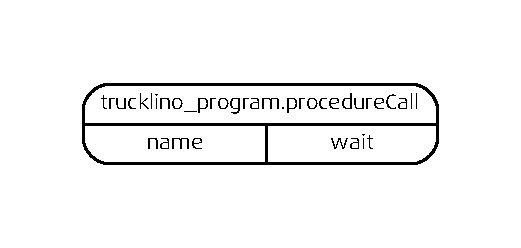
\includegraphics[width=\textwidth]{gfx/implementation-program-grammar-syntaxtree-tree-wait.graphviz.pdf}
    \caption{Syntaxbaum des Aufrufs der Prozedur \inlinec|wait|}
    \label{fig:implementation:datastructure:syntaxtree:1:wait}
  \end{subfigure}\hfill
  \begin{subfigure}[b]{0.45\textwidth}
    \includegraphics[width=\textwidth]{gfx/implementation-program-grammar-syntaxtree-tree-lightIsRed.graphviz.pdf}
    \caption{Syntaxbaum des Sensors \inlinec|lightIsRed|}
    \label{fig:implementation:datastructure:syntaxtree:1:lightIsRed}
  \end{subfigure}\hfill
  \caption{Prozeduraufruf \inlinec|wait| und Sensor \inlinec|lightIsRed|}
  \label{fig:implementation:datastructure:syntaxtree:1}
\end{figure}

Kinder von Knoten werden in benannten Kindgruppen organisiert. Dabei handelt es sich um eine Verallgemeinerung der von XML bekannten Aufteilung in Attribut-Kinder und Element-Kinder. Mit diesen Syntaxbäumen lassen sich die Kinder folglich beliebig in Unterbäumen organisieren~\cite[4]{riemer2018}. So sind die in Abbildung \ref{fig:implementation:datastructure:syntaxtree:1} abgebildeten Knoten in Abbildung \ref{fig:implementation:datastructure:syntaxtree:2} als Kindknoten einer kopfgesteuerten Schleife dargestellt, welche wiederum als Kindknoten des Wurzelknotens des Programms eingebunden ist. Nachdem die Abbruchbedingung der Schleife erfüllt ist, ist ein \inlinec|goForward|-Prozeduraufruf enthalten.

\begin{figure}[h]
  \centering
  \includegraphics[width=0.7\textwidth]{gfx/implementation-program-grammar-syntaxtree-tree-program.graphviz.pdf}
  \caption{Beispiel eines vollständigen Programms als Syntaxbaum}
  \label{fig:implementation:datastructure:syntaxtree:2}
\end{figure}

Die gezeigten Graphen dienen an dieser Stelle der Übersicht. Intern werden Syntaxbäume als JSON-Dokumente verwaltet.

Die Auswertung eines solchen Syntaxbaumes ist im folgenden Abschnitt beschrieben.

%************************************************
% Auswertung
%************************************************
\section{Auswertung}
\label{sec:implementation:evaluation}

Für die Auswertung und Ausführung des durch den Syntaxbaum beschriebenen Codes kommen zwei Vorgehensweisen infrage. In der Informatik bezeichnet der Begriff Kompilieren klassischerweise die Übersetzung von menschenfreundlichen Sprachelementen in maschinennahen Instruktionen, die von einem Prozessor und dem Betriebssystem verarbeitet werden können. Beim Interpretieren wird das Programm nicht vollständig übersetzt, sondern "portionsweise" analysiert, in eine zugehörige Folge von Prozessorinstruktionen übertragen und ausgeführt~\cite[47]{wagenknecht2009}. Da im Browser jedoch nicht direkt Maschinencode ausgeführt werden kann, ist der Unterschied in diesem Zusammenhang etwas anders zu verstehen:

\begin{itemize}
  \item Beim \emph{Interpretieren} wird der Syntaxbaum nach und nach durch ein in JavaScript geschriebenes Programm abgearbeitet und die entsprechenden Befehle direkt ausgeführt. In dieser Umgebung lässt sich der Fortschritt des Programms leicht verfolgen, da der Interpreter zu jedem Zeitpunkt die Position kennt, bis zu der der Code bisher ausgeführt wurde. Dies ermöglicht den Einbau von aussagekräftigen Debuggingfunktionen für den den auszuführenden Code. Außerdem ist es leicht möglich Mechanismen bereitzustellen, welche die Ausführung an einer beliebigen Stelle stoppen oder pausieren und später fortsetzen.
  \item Im Unterschied dazu ist \emph{Kompilieren} in diesem Zusammenhang so zu verstehen, dass ein JavaScript-Programm den Syntaxbaum zunächst in ein vollständig ausführbares JavaScript-Programm überführt. Der JavaScript-Code liegt bei diesem Vorgehen nach dem Kompilieren als String vor und kann anschließend als Ganzes in einer Art "Sandkasten" ausgeführt werden. Innerhalb dieser "Blackbox" lässt sich nur recht unzuverlässig auf den aktuellen Zustand des laufenden Programmes schließen ohne zusätzlichen Code einzufügen, der die Lesbarkeit des generierten Codes verschlechtert. Eben diese Lesbarkeit des generierten Codes ist aber einer der wichtigsten Vorteile dieser Vorgehensweise. Der Code lässt sich nicht nur für seine Ausführung nutzen, sondern kann gerade im Kontext einer Lernsoftware für den Nutzer interessant sein und ihm angezeigt werden.
\end{itemize}

Im Verlauf der Arbeit wurde die Vorgehensweise "Kompilieren" als Anforderung vorgegeben, da dieses Vorgehen speziell für BlattWerkzeug den Vorteil mit sich bringt, dass generierter Code in Zukunft vor der Ausführung dem Nutzer angezeigt und von ihm bearbeitet werden kann, was den Übergang zu einer Universalsprache erleichtern würde (siehe auch \ref{sec:conclusion:future}).

\subsection{Codegenerator}
\label{sec:implementation:evaluation:codegenerator}

Für die Kompilierung des Syntaxbaumes wird auf die von BlattWerkzeug zur Verfügung gestellten Codegenerator-Strukturen zurückgegriffen, die es ermöglichen, einen Codegenerator zu implementieren, der Übersetzungsregeln für jeden Knotentyp definiert. Abbildung \ref{fig:implementation:evaluation:codegenerator} zeigt die Implementierung eines Codegenerators für Knoten, die eine While-Schleife repräsentieren. Zwischen den Klammern innerhalb der \inlinec{while}-Anweisung wird der Kindknoten für die Bedingung der Schleife eingefügt, gefolgt vom Inhalt der Schleife. Diese Kindknoten werden wiederum durch ähnlich aufgebaute Generatoren umgewandelt bis der vollständige Code des Wurzelknotens im Syntaxbaum übersetzt wurde. Abbildung \ref{fig:implementation:evaluation:tree-render} zeigt den Ausschnitt eines Syntaxbaumes, welcher durch den Codegenerator in den in Abbildung \ref{fig:implementation:evaluation:tree-result} gezeigten Code kompiliert wird.

\begin{figure}
  \lstinputlisting{snippets/implementation-program-evaluation-codegenerator.ts}
  \caption{Implementierung des Codegenrator für eine Verzweigung}
  \label{fig:implementation:evaluation:codegenerator}
\end{figure}

\begin{figure}
  \centering
  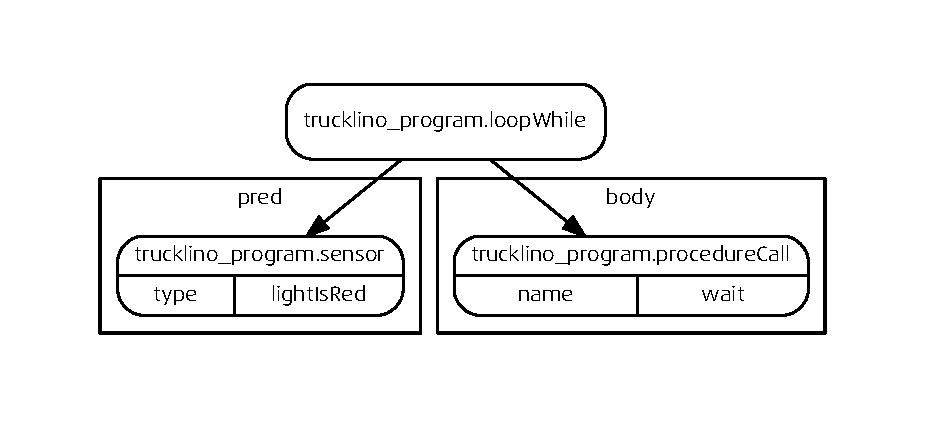
\includegraphics[width=\textwidth]{gfx/implementation-program-evaluation-tree.graphviz.pdf}
  \caption{Beispielhafter Ausschnitt eines Syntaxbaum für eine Verzweigung}
  \label{fig:implementation:evaluation:tree-render}
\end{figure}

\begin{figure}
  \lstinputlisting{snippets/implementation-program-evaluation-tree-result.js}
  \caption{Kompilierter Code für den Syntaxbaum in Abbildung \ref{fig:implementation:evaluation:tree-render}}
  \label{fig:implementation:evaluation:tree-result}
\end{figure}

\subsection[Umgebung zur Ausführung]{Umgebung zur Ausführung\protect\footnotemark}
\label{sec:implementation:evaluation:environment}

\footnotetext{Zum Verständnis dieses und folgender Abschnitte werden grundlegende Kenntnisse über die Konzepte von Promises, asynchronen Funktionen und Generatorfunktionen in JavaScript vorausgesetzt.}

Dem kompilierten Code muss zur Ausführung eine Umgebung bereitgestellt werden, welche die in Tabelle \ref{tbl:implementation:elements:cmds} gelisteten und als "atomaren Befehle" bezeichneten Funktionen, sowie Funktionen zur Ermittlung der Sensorwerte (siehe Tabelle \ref{tbl:implementation:elements:sensors}) zur Verfügung stellt. Für diese Aufgabe bietet sich der \inlinec{Function}-Konstruktor\footnote{\url{https://developer.mozilla.org/de/docs/Web/JavaScript/Reference/Global_Objects/Function}} an. Dieser Konstruktor transfomiert einen String in eine ausführbare JavaScript-Funktion. Im Gegensatz zu \inlinec{eval} ermöglicht der \inlinec{Function}-Konstruktor die Ausführung von Code im globalen Gültigkeitsbereich, was zu besseren Programmiergewohnheiten führt und eine effizientere Code-Minimierung ermöglicht~\cite{mdn-function}. In diesem speziellen Fall wird für die Ausführung des Codes der \inlinec{GeneratorFunction}-Konstruktor\footnote{\url{https://developer.mozilla.org/de/docs/Web/JavaScript/Reference/Global_Objects/GeneratorFunction}} verwendet (siehe dazu auch Abschnitt \ref{sec:implementation:rendering:animation}).

Für die Bereitstellung der Befehle und Sensoren werden im folgenden vier Varianten betrachtet. In Abbildung \ref{fig:implementation:environment} werden Implementationsbeispiele dieser Varianten einander gegenüber gestellt.

\begin{description}
  \item[1. Definition und Aufruf mit Enum-Klasse:] Eine Enum-Klasse mit allen Sensoren und Befehlen, sowie zwei Funktionen für deren Auswertung gibt es schon. Darauf aufbauend wäre eine nahe liegende Möglichkeit, diese Funktionen und die Enum-Klassen einfach in der Welt bereitzustellen. Ein deutlicher Vorteil dieser Lösung ist der geringe zusätzliche Implementierungsaufwand und die verbesserte Wartbarkeit. Kommen neue Befehle oder Sensoren dazu, stehen diese automatisch auch in der Umgebung zur Verfügung. Der generierte Code ist jedoch nicht intuitiv und sollte er dem Nutzer angezeigt werden, nicht besonders gut zu verstehen. Außerdem halten sich die Funktionsaufrufe nicht an gängige Muster, was den späteren Umstieg auf Universalsprachen erschweren könnte \fref{fig:implementation:environment:func}.
  \item[2. Definition und Aufruf mit \inlinec|call|:] Eine weitere denkbare Lösung ist es, ein Objekt mit allen benötigten Funktionen für Befehle und Sensoren zu erzeugen und dieses als Wert von \inlinec{this} innerhalb der Funktion zur Verfügung zu stellen. Selbstdefinierte Prozeduren werden innerhalb der Funktion ebenfalls als Kinder von \inlinec{this} definiert. Dieses Vorgehen hat den Vorteil, dass der Code deutlich intuitiver wird, als dies bei der vorgehend beschriebenen Variante der Fall wäre. Jedem Aufruf muss zwar ein \inlinec{this} vorangestellt werden, jeder Befehl hat aber seinen eigenen Funktionsaufruf. Der zusätzliche Implementierungsaufwand ist allerdings ein Nachteil dieser Variante. Es müssen in einem Objekt Wrapper-Funktionen für alle Befehle und Sensoren definiert werden. Kommt zu einem späteren Zeitpunkt ein Befehl oder ein Sensor hinzu, muss dieser zusätzlich auch an dieser Stelle hinzugefügt werden. Außerdem müssen selbst definierte Prozeduren mithilfe von Pfeilfunktionen\footnote{\url{https://developer.mozilla.org/de/docs/Web/JavaScript/Reference/Functions/Pfeilfunktionen}} definiert werden, damit der Bezug zum \inlinec{this} nicht verloren geht \fref{fig:implementation:environment:this}.
  \item[3. Definition und Aufruf über Parameter:] Auch wäre es möglich, alle Befehle und Sensoren als Parameter der Funktion zu definieren. Dadurch würde im Vergleich zur vorigen Variante die Notwendigkeit entfallen, \inlinec{this} vor jeden Aufruf zu stellen. Da die Wrapper-Funktionen in diesem Fall allerdings ebenfalls zusätzlich definiert werden müssen und die Zuordnung ihrer Namen fehleranfällig ist, birgt dieses Vorgehen abgesehen von dem etwas kompakteren Code, keine weiteren Vorteile \fref{fig:implementation:environment:param}.
  \item[4. Definition und Aufruf mit einem Objekt als Parameter:] Letztlich kommt auch eine Kombination der Varianten zwei und drei infrage, bei der alle Befehle und Sensoren in einem Objekt zusammengefasst werden. Im Vergleich zu Variante zwei muss das \inlinec{this} lediglich durch einen Variablennamen ersetzt werden. Dadurch ist es nun nicht zwingend erforderlich, Pfeilfunktionen für die Definition von benutzerdefinierten Prozeduren zu nutzen \fref{fig:implementation:environment:obj}.
\end{description}

Für den Einsatz in dieser Arbeit ist Variante vier am sinnvollsten, da so Wartbarkeit und Lesbarkeit des generierten Codes in einem angemessenen Verhältnis stehen. Außerdem werden Generatorfunktionen\footnote{\url{https://developer.mozilla.org/de/docs/Web/JavaScript/Reference/Statements/function*}} für die benuzterdefinierten Prozeduren verwendet, welche die Definition über Pfeilfunktionen nicht unterstützen. Der \inlinec{this}-Kontext würde bei Variante zwei dadurch verloren gehen.

Es wird also ein Objekt mit Wrapper-Funktionen für alle Befehle und Sensoren erzeugt und dieses als Parameter mit dem Namen \inlinec{truck} an die generierte Funktion übergeben. Die Bezeichnung \inlinec{truck} wurde gewählt, da alle Befehle aus Sicht des Trucks ausgeführt werden und \inlinec{truck.goForward()} sinnvoll lesbar sind.

\begin{figure}
  \begin{subfigure}[b]{\textwidth}
    \lstinputlisting{snippets/implementation-program-environment-func.js}
    \caption{Definition und Aufruf mit Enum-Klasse}
    \label{fig:implementation:environment:func}
    \vspace{0.5cm}
  \end{subfigure}
  \begin{subfigure}[b]{\textwidth}
    \lstinputlisting{snippets/implementation-program-environment-this.js}
    \caption{Definition und Aufruf mit \inlinec|call|}
    \label{fig:implementation:environment:this}
    \vspace{0.5cm}
  \end{subfigure}
  \begin{subfigure}[b]{\textwidth}
    \lstinputlisting{snippets/implementation-program-environment-param.js}
    \caption{Definition und Aufruf über Parameter}
    \label{fig:implementation:environment:param}
    \vspace{0.5cm}
  \end{subfigure}
  \begin{subfigure}[b]{\textwidth}
    \lstinputlisting{snippets/implementation-program-environment-obj.js}
    \caption{Definition und Aufruf mit einem Objekt als Parameter}
    \label{fig:implementation:environment:obj}
  \end{subfigure}
  \caption{Varianten für die Bereitstellung der Befehle und Sensoren innerhalb der generierten Funktion}
  \label{fig:implementation:environment}
\end{figure}

\subsection{Ausführungsdauer von Befehlen}
\label{sec:implementation:evaluation:execution-time}

Die Ausführung der atomaren Befehle wie dem des Vorwärtsfahren oder Warten haben in JavaScript aufgrund ihrer geringen Komplexität eine kaum merkliche Ausführungszeit. Um die Ausführung trotzdem sichtbar zu machen, soll diese Ausführungszeit künstlich erhöht werden können. Diese Eigenschaft ist unter anderem auch für die Animation in der Darstellung (siehe \ref{sec:implementation:rendering:animation}) von Bedeutung.

Zur Darstellung einiger Operationen wird eine gewisse Zeit benötigt. So ist für die Operation des Vorwärtsfahrens, ein Zeitschritt festgelegt, beim Setzen eines Blinkers kann die verbrauchte Zeit jedoch vernachlässigt werden, daher wird diese Operation mit null Zeitschritten bewertet. Die tatsächliche Zeit, die ein Zeitschritt verbraucht, kann separat festgelegt werden. Dadurch ist es möglich die Zeit (z.~B. für die Auswertung von Testfällen) kleiner zu stellen und dadurch die Ausführung schneller laufen zu lassen.

Auch sind die Zeitschritte für die Berechnung der Ampelphasen relevant. Für Ampeln kann die Dauer der Rot- und Grünphasen in Zeitschritten festgelegt werden. Eine Ampel mit einer Rotphase von einem Zeitschritt sowie einer Grünphase von ebenfalls einem Zeitschritt wird nun nach jeder Vorwärtsbewegung oder Aufruf des Warten-Befehls umspringen, jedoch nicht beim Wechsel der Blinkerseite.

Um der Ausführungszeit im Programmablauf gerecht zu werden, stellt die \inlinec{World}-Klasse neben der \inlinec{command}-Methode zusätzlich die Methode \inlinec{commandAsync} bereit, die als asynchrone Funktion definiert ist und ein \inlinec{Promise} zurückgibt, welches erfüllt wird, sobald die für diesen Befehl vorgesehene Zeit abgelaufen ist.

Um auch das Pausieren und Fortsetzen der Ausführung zu ermöglichen, kommt für die Ausführung des generierten Codes eine Generatorfunktion zum Einsatz (siehe \ref{sec:implementation:evaluation:pause}).

\subsection{Behandlung von Endlosschleifen}
\label{sec:implementation:evaluation:infinite-loop}

Im Vergleich zu Beginn dieses Abschnittes, wurde ein Vorteil der Vorgehensweise "Interpretieren" genannt, welcher gleichzeitig ein Nachteil beim Kompilieren darstellt: Wurde mit der Ausführung des kompilierten Codes einmal begonnen, kann diese nicht einfach unterbrochen werden. Dies stellt insbesondere ein Problem dar, wenn der Nutzer eine Endlosschleife in sein Programm eingebaut hat. Das Programm läuft im gleichen Kontext wie die Webseite und kann diese daher einfrieren. Um dieses Problem zu umgehen, wurde zusätzlich der \inlinec{doNothing}-Befehl eingeführt. Dieser Befehl steht im Drag \& Drop-Editor nicht zur Verfügung. Er verändert -- ähnlich wie der \inlinec{wait}-Befehl -- den Zustand der Welt nicht, fügt im Gegensatz zu \inlinec{wait} allerdings keinen neuen Zustand ein, kann also auch nicht rückgängig gemacht werden. Trotzdem erzeugt dieser Befehl eine für den Nutzer kaum merkliche Wartezeit von wenigen Millisekunden. Mit diesem Vorgehen kann aktives Warten ("busy waiting") beim Aufruf einer leeren While-Schleife und daraus resultierendes Blockieren der Bedienelemente von BlattWerkzeug vermieden werden.

Den \inlinec{doNothing}-Befehl nur in leeren Schleifen einzufügen, reicht nicht aus. Zwar wäre es möglich, vereinzelte Konstellationen zu überprüfen und auf den zusätzlichen Befehl zu verzichten, wenn eine andere Anweisung auf gleicher Ebene aufgerufen wird, allerdings wird dieses Vorgehen sehr aufwendig, wenn auch kompliziertere Strukturen wie z.~B. Verzweigungen oder untergeordnete Schleifen geprüft werden sollen. Dabei handelt es sich um eine Variante des Halteproblems. Es kann in vielen Fällen nicht sichergestellt werden, dass ein bestimmter Codepfad auch wirklich aufgerufen und der darin enthaltene Befehl ausgeführt wird.

Im nächsten Schritt ist es möglich, das Programm innerhalb einer Endlosschleife manuell vorzeitig zu beenden, bzw. zu pausieren.

\subsection{Vorzeitiges Beenden der Ausführung}
\label{sec:implementation:evaluation:pause}

Für das vorzeitige Beenden des Programms schien zunächst die Variante sinnvoll, dass zusätzlich innerhalb von allen Befehlen geprüft wird, ob der Nutzer die Beendigung des laufenden Programmes angewiesen hat. Ist dies der Fall, wird die Ausführung des aktuellen Codes durch den Wurf einer Exception vorzeitig beendet. Dieses Vorgehen ist eine Möglichkeit, die Ausführung des Codes vorzeitig zu beenden, ohne die Lesbarkeit durch zusätzliche Kontrollbefehle zu verschlechtern, hat allerdings die Nebenwirkung, dass \inlinec{try...catch}-Anweisungen in Zukunft nicht innerhalb des generierten Codes eingesetzt werden können. Außerdem ist es mit diesem Verhalten nicht möglich, das Programm an der Stelle fortzuführen, an der es gestoppt wurde, da der Kontext der Funktion mit dem Wurf der Exception verloren geht.

Dieses Problem wird mit der Nutzung von Generatorfunktionen umgangen. Der erzeugte Iterator führt in jedem Iterationsschritt einen Befehl aus und gibt das \inlinec{Promise} zurück, auf dessen Erfüllung gewartet wird, bevor in einer Schleife der nächste Iterationsschritt aufgerufen wird. Dies geschieht solange, bis alle Befehle im Programm abgearbeitet sind oder ein Flag innerhalb der \inlinec{World}-Klasse gesetzt wird, dass das Programm im nächsten Schritt pausiert werden soll. Da der Iterator gespeichert wird, kann im Falle eines Pausierens, die Ausführung an der Stelle fortgesetzt werden, an der sie stehen geblieben ist.

Im generierten Code muss dadurch allerdings jedem Funktionsaufruf ein \inlinec{yield*} vorangestellt werden. Außerdem müssen benutzerdefinierte Prozeduren ebenfalls als Generatorfunktionen definiert werden.

Die in den vorigen Abschnitten besprochene Datenstruktur, sowie die Elemente der Sprache benötigen nun eine geeignete Darstellung, deren Implementierung im nächsten Abschnitt diskutiert wird.

\subsection{Syntaxfehler}
\label{sec:implementation:syntax-errors}

Es kann nicht garantiert werden, dass der Code, welcher vom Codegenerator erzeugt wurde, frei von Syntaxfehlern ist. Dies kann aus der Kompilierung eines unvollständigen Syntaxbaumes resultieren. So kann es z.~B. vorkommen, dass die Bedingung bei einer While-Schleife leer ist. JavaScript wirft bei der Erzeugung der Funktion einen \inlinec{SyntaxError}. Um diesen Fehler abzufangen, muss die Erzeugung der Funktion innerhalb einer try...catch-Anweisung\footnote{\url{https://developer.mozilla.org/de/docs/Web/JavaScript/Reference/Statements/try...catch}} stattfinden \fref{fig:implementation:evaluation:try-catch}.

\begin{figure}
  \lstinputlisting{snippets/implementation-program-evaluation-try-catch.js}
  \caption{Möglicher Syntaxfehler innerhalb des generierten Codes}
  \label{fig:implementation:evaluation:try-catch}
\end{figure}

%************************************************
% Darstellung
%************************************************
\section{Darstellung}
\label{sec:implementation:rendering}

Erst die Darstellung in einer Mikrowelt erweckt die Minisprache zum Leben. Im Folgenden wird die Implementierung der Darstellung der zuvor definierten Datenstruktur beschrieben.

\subsection{Technologie}
\label{sec:implementation:rendering:technology}

Als mögliche Technologien für die Darstellung und Animation der Welt im Browser wurden vier Ansätze evaluiert. Eine Übersicht der Eigenschaften findet sich in Tabelle \ref{tbl:implementation:rendering:technology}.

\begin{itemize}[noitemsep]
  \item Rendering über klassische \emph{HTML}-Elemente und Styling mittels CSS und Integration von nachgeladenen Bilddateien.
  \item Rendering mittels eines eingebetteten \emph{SVG}-Elements.
  \item Rendering mittels eines \emph{Canvas}-Elements und Integration von nachgeladenen Bilddateien.
  \item Einsatz von \emph{WebGL} für die Darstellung einer dreidimensionalen Welt.
\end{itemize}

WebGL ist als Technologie für diese Arbeit als zu mächtig einzustufen. Die Erstellung von dreidimensionalen Modellen hätte den Rahmen dieser Arbeit gesprengt und -- abgesehen von einer möglichen schöneren Darstellung -- im Vergleich zu den übrigen Technologien keinen nennenswerten Nutzen gehabt.

Rendering mittels HTML oder SVG hat den Vorteil, dass sie sehr von den Funktionen des Angular-Framework profitieren. Die Datenstruktur kann direkt an HTML und SVG-Elemente angebunden werden und Angular kümmert sich um die Aktualisierung des DOM. Dieses Vorgehen reduziert den Aufwand für die Implementierung des Renderers enorm. Zusätzlich bringt Angular nativ ein Animationsframework mit. Für die Implementierung eines Prototyps wurde das Rendering mittels eines SVG-Element gewählt, da es gegenüber einfachem HTML den Vorteil bietet, Grafiken direkt und ohne zusätliches Nachladen von Ressourcen integrieren zu können.

In der Implementierung des Prototyps erwies sich allerdings das Animationsframework als ein Nachteil dieser Technologie. Angular setzt an dieser Stelle auf ein zustandsbasiertes System. Eine Animation findet immer zwischen zwei definierten Zuständen statt. Zustände können bestimmte CSS Regeln angeben, zwischen denen bei einem Zustandswechsel interpoliert wird~\cite{angular-animations}. Dieses System ist mit den Anforderungen, die der im Rahmen dieser Arbeit behandelte Anwendungsfall stellt, nicht kompatibel. Für die Animation eines Lastwagens müsste vielmehr zwischen verschiedenen Positionen interpoliert werden. Diese variablen Positionen lassen sich nicht sinnvoll auf fest definierte Zustände in Angular abbilden. Es müssten Zustände für jede Position des Lastwagens in jeder Drehung definiert werden.

So setzt die aktuelle Version des Programms auf einen Renderer mittels Canvas-Element. Dass Angular keine Funktionen zum Rendern in einem Canvas-Element bereithält und dieser Prozess vollständig außerhalb und unabhängig von Angular stattfinden muss, erwies sich schnell als ein Vorteil dieser Technologie. Der Renderer hat dadurch keine externen Abhängigkeiten, ermöglicht eine leichte Integration in BlattWerkzeug und könnte potenziell auch in eine Anwendung portiert werden, welche Angular nicht einsetzt. Der Nachteil, dass das Canvas in jedem Frame vollständig neu gezeichnet werden muss, wäre technisch zu umgehen, indem Bereiche ermittelt werden, die sich im Vergleich zum letzten Frame geändert haben und nur diese Bereiche neu gezeichnet werden. Auf die Implementierung dieses Verhaltens wurde allerdings in diesem Fall verzichtet, da aufgrund der geringen Komplexität der zu zeichnenden Grafik zu erwarten ist, dass moderne Computer keinerlei Schwierigkeiten beim ständigen Neuzeichnen des Bildes haben werden und die angesprochene Technik nicht trivial umzusetzen ist.

\begin{table}
  \centering
  \begin{tabular}{l|c|c|c|c}
                                      & HTML   & SVG    & Canvas & WebGL  \\ \hline
    Direkte Integration in Angular    & \cmark & \cmark & \xmark & \xmark \\ \hline
    Frameweises Rendering             & \xmark & \xmark & \cmark & \cmark \\ \hline
    Nachladen von Ressourcen notwenig & \cmark & \xmark & \cmark & \cmark \\ \hline
    Abhängigkeitsfrei                 & \xmark & \xmark & \cmark & \cmark \\ \hline
    Komplexe 3D-Modellen notwendig    & \xmark & \xmark & \xmark & \cmark \\ \hline
  \end{tabular}
  \vspace{5pt}
  \caption{Vergleich der Darstellungstechnologien}
  \label{tbl:implementation:rendering:technology}
\end{table}

\subsection{Objektstruktur}
\label{sec:implementation:rendering:structure}

Für das effektive Zeichnen der Welt auf einem Canvas-Element wurde eine Renderer-Klasse mit einer am Besucher-Schema orientierten Objektstruktur entwickelt, welche die einzelnen Elemente der Objektstruktur der Welt (siehe \ref{sec:implementation:structure}) zeichnet.

Die Objektstruktur des Renderers ist in \figreft{sec:implementation:rendering:structure:uml} zur besseren Übersicht vereinfacht dargestellt. Wurzelklasse ist hier der Renderer, welcher mit einem \inlinec{World}-Objekt (diese Objektstruktur wurde in Abschnitt \ref{sec:implementation:structure} beschrieben) und einem Canvas-Context instanziiert wird. Mit dem Aufruf der \inlinec{render}-Methode wird der Render-Prozess gestartet. Diese Methode zeichnet den Canvas-Inhalt und ruft sich mittels der \inlinec{requestAnimationFrame}-Funktion\footnote{\url{https://developer.mozilla.org/en-US/docs/Web/API/window/requestAnimationFrame}} immer wieder selbst auf.

Die Eigentliche Zeichenaufgabe gibt die \inlinec{Renderer}-Klasse jedoch an einen Baum von \inlinec{ObjectRenderer}-Klassen ab, die für die Darstellung wesentlicher visueller Objekte zuständig sind. Die Struktur der \inlinec{ObjectRenderer} ist an der Weltobjektstruktur orientiert. Die \inlinec{Renderer}-Klasse hält eine Instanz eines \inlinec{WorldRenderer}, welcher die von ihm gehaltene \inlinec{WorldStateRenderer}-Instanz über Zustandsänderungen der Welt informiert. Der \inlinec{WorldStateRenderer} verwaltet genau eine \inlinec{TruckRenderer}-Instanz, welche für das letztendliche Zeichnen des Lastwagens und die Animation von dessen Zustandsübergängen verantwortlich ist, sowie die notwendige Anzahl von \inlinec{TileRenderer}-Instanzen. Die \inlinec{draw}-Methode der \inlinec{ObjectRenderer} werden immer mit einem \inlinec{RenderingContext} aufgerufen, welcher den Zeitstempel der Animation verwaltet, einen Verweis auf den zu verwendenden Canvas-Context enthält, sowie einige Hilfsmethoden zum Zeichnen bereitstellt.

Das sichtbare Bild wird durch die \inlinec{ObjectRenderer} vollständig aus verschiedenen Komponenten zusammengesetzt, die aus SVG-Sprites an die richtige Stelle im Bild gezeichnet werden. Die Hintergründe der Straßen stammen aus einer freien Sammlung von Spielegrafiken\footnote{\url{https://opengameart.org/node/16589}}, der Truck und die Fracht wurden für den Zweck dieser Arbeit selbst gezeichnet. Alle 16 Varianten von Kacheln sind im Sprite verfügbar. Lediglich der Truck muss vor dem Zeichnen in die richtige Richtung gedreht werden. Ein Vorbereiten aller möglichen Drehungen des Lastwagens im Sprite ist an dieser Stelle nicht sinnvoll, da die Drehung des Lastwagens animiert interpoliert werden soll.

\begin{figure}
  \begin{tikzpicture}
  \tikzstyle{every node}=[font=\small]

  \begin{class}[text width=7cm]{Renderer}{1,0}
    \attribute{running: boolean}

    \operation{constructor(world: World, ctx: CanvasContext)}
    \operation{stop()}
    \operation{render(timestamp: TimeStamp)}
  \end{class}

  \begin{class}[text width=5cm]{RenderingContext}{9,0}
    \attribute{ctx: CanvasRenderingContext2D}
    \attribute{width: number}
    \attribute{height: number}
    \attribute{start: TimeStamp}
    \attribute{previousFrame: TimeStamp}
    \attribute{currentFrame: TimeStamp}

    \operation{animationSpeed(): number}
  \end{class}

  \begin{interface}[text width=5cm]{ObjectRenderer}{3.5,-3}
    \operation{draw(ctx: RenderingContext)}
  \end{interface}

  \begin{class}[text width=3cm]{WorldRenderer}{-1,-5}
    \implement{ObjectRenderer}

    \attribute{world: World}

  \end{class}

  \begin{class}[text width=4cm]{WorldStateRenderer}{-0.5,-7.5}
    \implement{ObjectRenderer}

    \attribute{state: WorldState}
    \attribute{freightTarget: Freight}

    \operation{update(state: WorldState)}
  \end{class}

  \begin{class}[text width=2.75cm]{TileRenderer}{5.5,-6}
    \implement{ObjectRenderer}

    \attribute{tile: Tile}

    \operation{update(tile: Tile)}
  \end{class}

  \begin{class}[text width=3.5cm]{TruckRenderer}{9.75,-7}
    % \implement{ObjectRenderer}

    \attribute{truck: Truck}
    \attribute{prevTruck: Truck}
    \attribute{initial: number}

    \operation{update(truck: Truck)}
  \end{class}

  \composition{Renderer}{ctx}{1}{RenderingContext}
  \composition{Renderer}{worldRenderer}{1}{WorldRenderer}
  \composition{WorldRenderer}{stateRenderer}{1}{WorldStateRenderer}
  \composition{WorldStateRenderer}{truckRenderer}{1}{TruckRenderer}
  \composition{WorldStateRenderer}{tileRenderers}{0..*}{TileRenderer}

  \draw[umlcd style implement line](ObjectRenderer) -- (TruckRenderer.north);
\end{tikzpicture}

  \caption{Vereinfachtes UML-Diagramm der Rendererobjektstruktur}
  \label{sec:implementation:rendering:structure:uml}
\end{figure}

\subsection{Zielerfüllung}
\label{sec:implementation:finish}

Hat der Nutzer mit seinem Programm oder aber manuell über die Befehlbuttons alle Container an ihr Ziel verbracht, erkennt die Software, dass das Spielfeld gelöst ist. Der Nutzer erhält eine Statusmeldung, dass das Spielfeld gelöst wurde, wird aber nicht aus der aktuellen Arbeitsumgebung herausgerissen. Vielmehr soll er die Möglichkeit bekommen, das eigene Programm noch einmal zu lesen und zu verstehen, \emph{warum} dieses Programm zu der Lösung geführt hat. Außerdem kann der Nutzer so sein Programm weiter optimieren und vielleicht eine Lösung implementieren, welche noch schneller zum gewünschten Ergebnis führt. Einzelne Schritte können dafür mithilfe eines entsprechenden Buttons rückgängig gemacht werden, oder aber die Welt wird direkt wieder auf ihren Ausgangszustand zurückgesetzt.

\subsection{Level-Editor}
\label{sec:implementation:level-editor}

Für den Drag \& Drop-Editor wurde eine weitere Grammatik in BlattWerkzeug eingeführt, welche es ermöglicht, eine eigene Karte zu kreieren. Der hieraus generierte Syntaxbaum wird in eine Beschreibung einer Welt (\inlinec{WorldDescription}) umgewandelt, mit der die \inlinec{World}-Klasse instanziiert werden kann. Abbildung \ref{fig:implementation:level-editor:tree} zeigt auschnittsweise einen beispielhaften Syntaxbaum für eine Welt. Diese Beschreibung enthält sowohl die Größe der Welt, sowie die Position und initiale Beladung des Lastwagens, als auch eine Liste von Kacheln, welche wiederum ihre Position definieren und Informationen über Ampeln, Fracht und Frachtziele enthalten.

Für die Aufgabe der Definition einer umfangreichen listenartigen Datenstruktur wie der einer Welt, erwies sich der Drag \& Drop-Editor als eher ungeeignet. Der Nutzer muss ein sehr genaues Bild der Welt vor Augen haben, um die Kacheln mit den richtigen Öffnungen zu platzieren. Um die Welten für die Beispielaufgaben besser erzeugen zu können, wurde ein rudimentärer Level-Editor entwickelt, der als JavaScript-Anwendung unabhängig von BlattWerkzeug funktioniert und den Syntaxbaum der Welt ausgibt. Dieser muss anschließend manuell in die BlattWerkzeug-Datenbank einkopiert werden. Da dies keine Lösung für reguläre Anwender darstellt und damit Lehrer ohne tiefer gehende Kenntnisse der Software in Zukunft selbst in der Lage sind, eigene Aufgabenstellungen vorzubereiten, wäre die Entwicklung eines geeigneten Level-Editors innerhalb der BlattWerkzeug-Umgebung, aber unabhängig vom Drag \& Drop-Editor, notwendig. In Absprache mit den Gutachtern wurde dieser Ansatz aus Zeitgründen nicht weiter verfolgt.

\begin{figure}
  \lstinputlisting{snippets/implementation-program-level-editor-tree.json}
  \caption{Beispielhafter Syntaxbaum einer Welt (verkürzt)}
  \label{fig:implementation:level-editor:tree}
\end{figure}

\subsection{Lastwagen-Position}
\label{sec:implementation:rendering:truck-position}

Sowohl bei Kara \tref{sec:related:kara}, als auch bei Lightbot \tref{sec:related:lightbot} bewegt sich die Spielfigur von einer Kachel des Spielfeldes zur nächsten und kommt zwischen den Schritten auf der Mitte der Kachel zum Stehen. Eine Drehung findet auf der Stelle statt. Die Spielfigur dreht sich um sich selbst und kann sich auf diese Weise in alle vier Richtungen bewegen. So liegt es nahe, diese Verhalten auch für den Lastwagen zu implementieren \fref{fig:implementation:rendering:truck-position:diff:a}, jedoch ist zu bedenken, dass die Spielfiguren von Kara und Lightbot sich in einem realen Umfeld anders bewegen als ein Lastwagen. Während eine Drehung auf der Stelle für einen Marienkäfer und einen hüpfenden Roboter kein Problem darstellen, wäre der Fahrer eines Lastwagens mit dieser Aufgabe wohl überfordert. Ein Lastwagen dreht sich nur dann, wenn bei einer Vorwärtsbewegung die Lenkung eingeschlagen wird.

Um dieses Verhalten auch in die Mikrowelt zu übertragen, wurde eine Implementierung gewählt, bei der der Lastwagen auf der Kante der Kachel zum Stehen kommt. An dieser Stelle hat der Spieler die Möglichkeit, einen Blinker nach rechts oder links zu setzen und damit die Richtung bei der nächsten Vorwärtsbewegung zu beeinflussen \fref{fig:implementation:rendering:truck-position:diff:b}. Im Gegensatz zur erstgenannten Methode ist mit diesem Ansatz kein Wenden möglich. Der Lastwagen muss eventuell einen Umweg fahren, um sein Ziel zu erreichen und darf sich in keine Sackgassen begeben. Für die Zukunft wäre es allerdings denkbar, einen Rückwärtsgang einzuführen.

\begin{figure}
  \begin{subfigure}[b]{0.45\textwidth}
    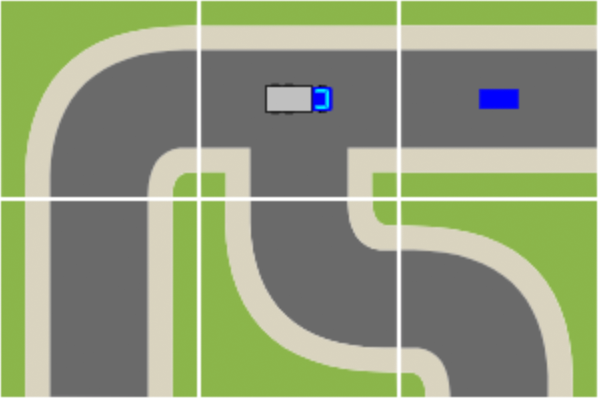
\includegraphics[width=\textwidth]{gfx/implementation-rendering-truck-position-diff-a.png}
    \caption{Haltepunkt auf der Mitte der Kachel}
    \label{fig:implementation:rendering:truck-position:diff:a}
  \end{subfigure}\hfill
  \begin{subfigure}[b]{0.45\textwidth}
    \includegraphics[width=\textwidth]{gfx/implementation-rendering-truck-position-diff-b.png}
    \caption{Haltepunkt auf der Kante der Kachel}
    \label{fig:implementation:rendering:truck-position:diff:b}
  \end{subfigure}\hfill
  \caption{Haltepunkte des Lastwagen im Spielfeld (zur besseren Erkennbarkeit sind die Kanten der Kacheln hervorgehoben)}
  \label{fig:implementation:rendering:truck-position:diff}
\end{figure}

\subsection{Animationsschritte}
\label{sec:implementation:rendering:animation}

Durch Animationen kann das Benutzererlebnis noch einmal deutlich aufgewertet werden, indem sie den Ausführungsfluss der Anwendung verlangsamen und dadurch die Nachvollziehbarkeit der ausgeführten Befehle ermöglicht wird. Zwischen den Positionen des Lastwagens wird daher zeitlich interpoliert. Eine wichtige Grundlage dafür wurde mit der Welt-Objektstruktur bereits geschaffen \tref{sec:implementation:structure}: Jede Operation erzeugt einen neuen Zustand, der in einer Liste gespeichert wird. Dieses Vorgehen macht es leicht zwischen dem aktuellen und dem vorherigen Zustand zu interpolieren.

Auch die in Abschnitt \ref{sec:implementation:evaluation:execution-time} beschriebenen Zeitschritte spielen an dieser Stelle eine wesentliche Rolle. Eine Animation der Bewegung des Lastwagens wird so z.~B. immer im Zeitraum eines Zeitschrittes animiert. Dadurch, dass die Ausführung des Programms genau diese Dauer als Ausführungszeit vorsieht, entsteht eine flüssige, nachvollziehbare Animation über mehrere Zeitschritte hinweg.

%************************************************
% Integration
%************************************************
\section[Integration]{Integration\protect\footnotemark}
\label{sec:implementation:integration}

\footnotetext{Zum Verständnis dieses Abschnittes werden grundlegende Kenntnisse über Angular (insbesondere Services und Komponenten) vorausgesetzt.}

Um mit möglichst wenigen Abhängigkeiten und dadurch geringerem Zeitaufwand verschiedene Ansätze ausprobieren zu können, wurde zunächst mit der Entwicklung eines Prototypen auf einer "grünen Wiese" begonnen. Auch wenn der Prototyp als Angular-Anwendung aufgesetzt wurde, erfolgte der Großteil der Entwicklung außerhalb dieser Umgebung. Nachdem der ursprüngliche Ansatz der Darstellung mittels SVG-Grafiken verworfen und die Darstellung auf Canvas-Rendering umgestellt wurde, sind die Objektstruktur, sowie der Renderer vollständig unabhängig von Angular implementiert, da sie von den von Angular bereitgestellten Strukturen nicht profitieren können. Diese Klassen konnten so ohne Anpassungen in die Umgebung von BlattWerkzeug übernommen werden. Lediglich die rudimentäre Benutzeroberfläche des Prototypen (siehe Abbildung \ref{fig:implementation:integration:prototype}) wurde mithilfe von Angular umgesetzt, für die Integration in BlattWerkzeug in dieser Form jedoch nicht mehr benötigt.

\begin{figure}
  \centering
  \includegraphics[width=0.4\textwidth]{gfx/implementation-integration-prototype.png}
  \caption{Bildschirmfoto der UI des Prototyp vor der Integration in BlattWerkzeug}
  \label{fig:implementation:integration:prototype}
\end{figure}

\subsection{Angular-Service}
\label{sec:implementation:integration:ng-service}

Ein Projekt in BlattWerkzeug kann sowohl mehrere Welten, als auch mehrere Programme beinhalten. Diese zusammenzubringen ist die Aufgabe des \inlinec{TruckWorldService}. Die Auslagerung dieser Funktionalität ist notwendig, da Darstellung und Steuerung der Welten über mehrere Angular-Komponenten verteilt sind. Alle diese Komponenten erhalten in Abhängigkeit des aktuell geöffneten Programmes die entsprechende Instanz der Welt. Auch übernimmt der Service die Aufgabe -- falls notwendig -- eine neue Instanz einer Welt zu erzeugen.

Eine besondere Schwierigkeit ist in diesem Zusammenhang die Zuordnung einer Welt zu einem Programm. BlattWerkzeug bietet aktuell nicht die Möglichkeit, eine Verknüpfung zwischen verschiedenen Ressourcen herzustellen. Zu diesem Zweck wurde eine Auswahlbox implementiert, welche in die UI der Controller-Komponente (siehe nächstes Kapitel) eingegliedert wurde und in einem Auswahlfeld alle im aktuellen Projekt verfügbaren Welten darstellt. Die Auswahl wird an den \inlinec{TruckWorldService} weitergegeben, der sie zwischenspeichert. So geht die Auswahl der Welt, sowie deren aktueller Zustand auch nicht verloren, wenn der Nutzer zwischen verschiedenen Programmen wechselt. Aufgrund der fehlenden Speichermöglichkeit in BlattWerkzeug, muss die Welt allerdings erneut ausgewählt werden, sobald die Seite neu geladen, und der Service dadurch neu instanziiert wird.

\subsection{Komponenten}
\label{sec:implementation:integration:components}

Innerhalb der UI von BlattWerkzeug werden die Funktionen dieser Erweiterung mithilfe von Komponenten dargestellt. Eine Übersicht der im Folgenden beschriebenen Komponenten findet sich in Abbildung \ref{fig:implementation:integration:components}.

An dieser Stelle soll bemerkt werden, dass die Sidebar, von der sich die einzelnen Befehle, Sensoren und anderen Elemente der Sprache in das Programm ziehen lassen, bewusst auf Deutsch gehalten ist, während die Befehle im Programm analog zu JavaScript in englischer Sprache gehalten sind. Dadurch soll der Nutzer von Anfang an mit dem Eindruck von Code vertraut gemacht werden, während er durch die deutschen Begriffe in Sidebar bei der Wahl der sprachlichen Elemente unterstützt wird.

\begin{figure}
  \centering
  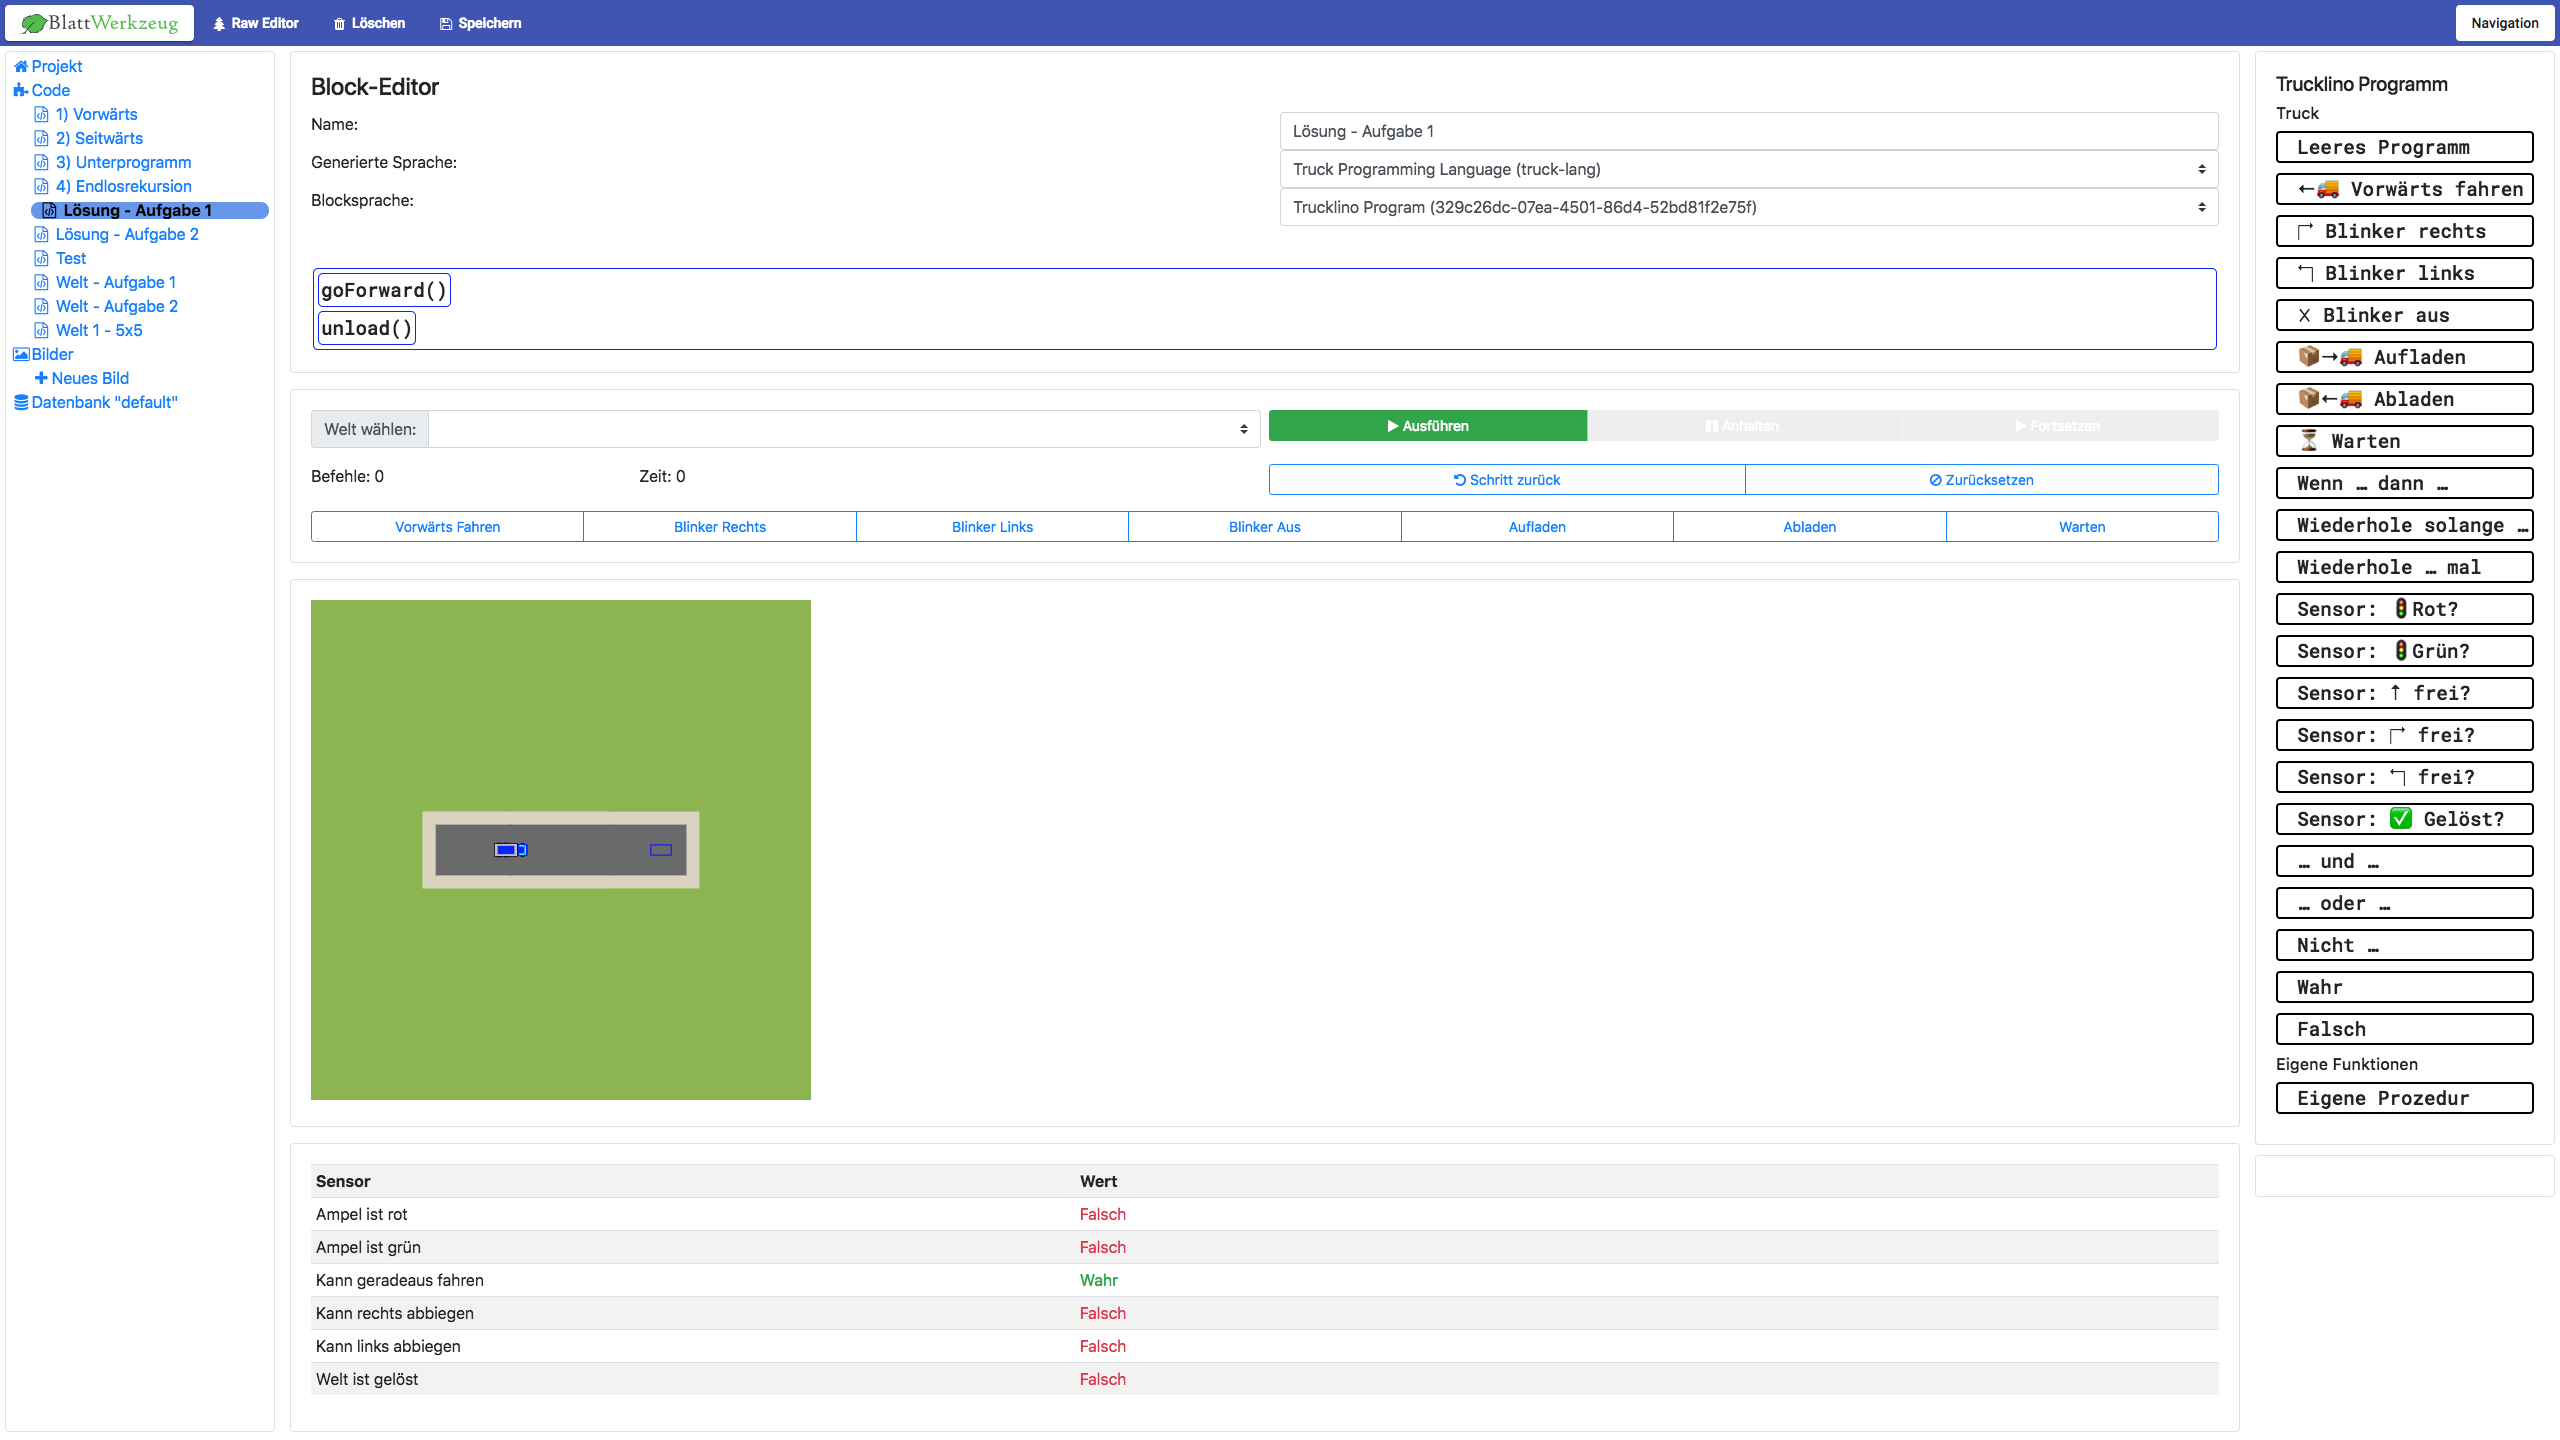
\includegraphics[width=1.0\textwidth]{gfx/implementation-integration-components.png}
  \caption{Bildschirmfoto der Komponenten in der UI von BlattWerkzeug}
  \label{fig:implementation:integration:components}
\end{figure}

\subsubsection{Renderer}
\label{sec:implementation:integration:renderer}

Zum Anzeigen der Welt wurde in BlattWerkzeug eine Komponente definiert, welche die \inlinec{Renderer}-Klasse (siehe \ref{sec:implementation:rendering:structure}) aus dem Prototypen nahezu ohne Anpassungen übernehmen konnte. Die Komponente erhält vom \inlinec{TruckWorldService} die aktuelle \inlinec{World}-Instanz, mit der sie den Renderer instanziiert und außerhalb der Angular Zone den Renderingprozess startet. Diese Komponente greift dabei lediglich lesend auf die Welt zu und nimmt keine Veränderungen vor.

Da der Renderingprozess bis zu 60 Mal in der Sekunde mittels \inlinec{requestAnimationFrame} ausgeführt wird, würde Angular andernfalls auch bis zu 60 Änderungserkennungen durchlaufen. Da keine Änderungen am Zustand vorgenommen werden, wäre dies in jedem Fall ergebnislos. Durch das Ausführen des Renderingprozesses außerhalb der Angular Zone, wird dies umgangen und die Performance kann gesteigert werden.

Zusätzlich wird die Komponente im Welt-Editor verwendet, um die bisher erstellte Welt darzustellen. Aus diesem Grund wurde darauf geachtet, die Darstellung möglichst robust und fehlertolerant zu gestalten, damit auch halb fertige Welten zuverlässig dargestellt werden können.

\subsubsection{Controller}
\label{sec:implementation:integration:controller}

Innerhalb der Controller-Komponente ist es möglich, die Befehle in der aktuellen Welt mithilfe von entsprechenden Buttons von Hand auszuführen. Außerdem kann an dieser Stelle die Ausführung des im Drag \& Drop-Editor zusammengestellten Programms gestartet und gestoppt werden. Es ist des Weiteren möglich, einzelne Befehle rückgängig zu machen oder die Welt direkt auf ihren Ausgangszustand zurückzusetzen.

Auch diese Komponente greift auf den \inlinec{TruckWorldService} zurück, um die aktuell gewählte Welt zu erhalten. Klicks auf die Buttons werden direkt an die entsprechenden Funktionen der \inlinec{World}-Klasse weitergeleitet.

Unter Verwendung des \inlinec{CurrentCodeResourceService}, einem von BlattWerkzeug bereitgestellten Service zum Erhalt der aktuellen Coderessource, kann auf den aus dem Drag \& Drop-Editor kompilierten Code zugegriffen werden. Dieser Code wird beim Klick auf den entsprechenden Button an die \inlinec{World}-Klasse zur Ausführung übergeben.

Solange eine Operation auf der Welt ausgeführt wird, sind die Bedienelemente zur Ausführung weiterer Befehle gesperrt. Erst nach Beendigung der Operation und damit auch der Animation, kann ein weiterer Befehl ausgeführt werden. Dazu existiert in der \inlinec{World}-Klasse ein Flag, welches während der Ausführung gesetzt und von dieser Komponente ständig ausgewertet wird.

\subsubsection{Sensoren}
\label{sec:implementation:integration:sensors}

Die Sensor-Komponente dient lediglich der Darstellung der aktuellen Werte aller Sensoren. Dadurch wird dem Nutzer im Navigationsmodus ermöglicht, sich in die Lage des Programms hineinzuversetzen und Entscheidungen basierend auf dem Wert von Sensoren zu treffen. Auch diese Komponente erhält über den \inlinec{TruckWorldService} Zugriff auf die aktuelle Welt, auf welche sie allerdings nur lesend zugreift.

%************************************************
% Zusammenfassung
%************************************************
\section{Zusammenfassung}
\label{sec:implementation:summary}

Dieses Kapitel beschreibt die Implementierung der im Rahmen dieser Arbeit entwickelten Erweiterung. In der Rahmenhandlung wird ein Lastwagen durch ein Netz von Straßen bewegt und löst Aufgaben, indem er farbige Container an ihre Ziele bringt.

Eine Objektstruktur verwaltet die Zustände der Mikrowelt, in der sich der Lastwagen bewegt. Gesteuert wird er durch den Nutzer mit Befehlen einer Minisprache, die mit ihrem reduzierten Umfang eine verständliche Einführung in verschiedene Konzepte wie Prozeduren, Schleifen und Verzweigungen gibt.

Die mit dem Drag \& Drop-Editor von BlattWerkzeug erstellten Programme werden in JavaScript Code übersetzt und die Ausführung in einer animierten Welt in einem Canvas-Element dargestellt. Ein zunächst entwickelter Prototyp wurde in Form eines Service und mehrerer Komponenten in das bestehende BlattWerkzeug-Projekt integriert.



%\appendix{}

%************************************************
% Literaturverzeichnis
%************************************************
\chapter{Literaturverzeichnis}
{%
\setstretch{1.1}
\renewcommand{\bibfont}{\normalfont\small}
\setlength{\biblabelsep}{0pt}
\setlength{\bibitemsep}{0.5\baselineskip plus 0.5\baselineskip}
% \printbibliography
\printbibliography[heading=none,title=Literaturverzeichnis,nottype=online]
\printbibliography[heading=subbibliography,title={Quellen im Internet},type=online,prefixnumbers={@}]
}
\cleardoublepage

%%************************************************
% Beispielaufgaben
%************************************************
\chapter{Beispielaufgaben}
\label{sec:exercises}

Die Anwendungsmöglichkeiten der Software sollen im Folgenden durch eine Reihe von Beispielaufgaben verdeutlicht werden. Die Aufgaben sind nicht geeignet von Schülern alleine gelöst zu werden. Es bedarf einer ausführlichen Einführung und die in den Aufgaben benötigten Konzepte müssen vorab durch eine Lehrkraft erklärt werden. Zusätzlich zum Bildschirmfoto der Musterlösung steht ein Video zur Verfügung, indem die Musterlösung gebaut und ausgeführt wird. Die Musterlösungen stellen i.~d.~R. nur eine von vielen Wegen dar die Aufgabe zu lösen.

\section{Aufgabe 1}
\label{sec:exercises:1}

Dein Lastwagen ist bereits beladen. Fahre zum Ablageplatz und lade den Container ab. Löse die Aufgabe, indem Du zwei Befehle hintereinander ausführst.

\begin{description}[noitemsep]
  \item[Welt wählen:] Welt A
  \item[Du brauchst:] Befehle
  \item[Video:] \url{https://vimeo.com/315544834} (Passwort: trucklino)
\end{description}

\begin{figure}[H]
  \begin{subfigure}[b]{0.40\textwidth}
    \includegraphics[width=\textwidth]{gfx/exercises-world-a.png}
    \caption{Welt A}
  \end{subfigure}\hfill
  \begin{subfigure}[b]{0.40\textwidth}
    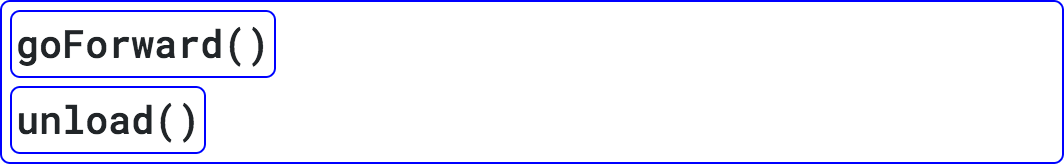
\includegraphics[width=\textwidth]{gfx/exercises-program-1.png}
    \caption{Musterlösung zu Aufgabe 1}
  \end{subfigure}\hfill
  \caption{Welt und Musterlösung zu Aufgabe 1}
\end{figure}

\pagebreak

\section{Aufgabe 2}
\label{sec:exercises:2}

Dieses Mal musst Du die Fracht erst aufladen. Dein Weg enthält außerdem eine Kurve. Reihe mehrere Befehle aneinander, um die Aufgabe zu lösen.

\begin{description}[noitemsep]
  \item[Welt wählen:] Welt B
  \item[Du brauchst:] Befehle
  \item[Video:] \url{https://vimeo.com/315545287} (Passwort: trucklino)
\end{description}

\begin{figure}[H]
  \begin{subfigure}[b]{0.40\textwidth}
    \includegraphics[width=\textwidth]{gfx/exercises-world-b.png}
    \caption{Welt B}
  \end{subfigure}\hfill
  \begin{subfigure}[b]{0.40\textwidth}
    \includegraphics[width=\textwidth]{gfx/exercises-program-2.png}
    \caption{Musterlösung zu Aufgabe 2}
  \end{subfigure}\hfill
  \caption{Welt und Musterlösung zu Aufgabe 2}
\end{figure}

\pagebreak

\section{Aufgabe 3}
\label{sec:exercises:3}

Erkennst Du das Muster? Wenn Du Deine Befehle in einer Prozedur verpackst, bleibt Dein Programm kurz und übersichtlich.

\begin{description}[noitemsep]
  \item[Welt wählen:] Welt C
  \item[Du brauchst:] Befehle, eigene Prozeduren
  \item[Video:] \url{https://vimeo.com/315545769} (Passwort: trucklino)
\end{description}

\begin{figure}[H]
  \begin{subfigure}[b]{0.40\textwidth}
    \includegraphics[width=\textwidth]{gfx/exercises-world-c.png}
    \caption{Welt C}
  \end{subfigure}\hfill
  \begin{subfigure}[b]{0.40\textwidth}
    \includegraphics[width=\textwidth]{gfx/exercises-program-3.png}
    \caption{Musterlösung zu Aufgabe 3}
  \end{subfigure}\hfill
  \caption{Welt und Musterlösung zu Aufgabe 3}
\end{figure}

\pagebreak

\section{Aufgabe 4}
\label{sec:exercises:4}

Deine Prozedur kannst Du auch in einer Zählerschleife mehrmals hintereinander ausführen.

\begin{description}[noitemsep]
  \item[Welt wählen:] Welt C
  \item[Du brauchst:] Befehle, eigene Prozeduren, Zählerschleife
  \item[Video:] \url{https://vimeo.com/315545858} (Passwort: trucklino)
\end{description}

\begin{figure}[H]
  \begin{subfigure}[b]{0.40\textwidth}
    \includegraphics[width=\textwidth]{gfx/exercises-world-c.png}
    \caption{Welt C}
  \end{subfigure}\hfill
  \begin{subfigure}[b]{0.40\textwidth}
    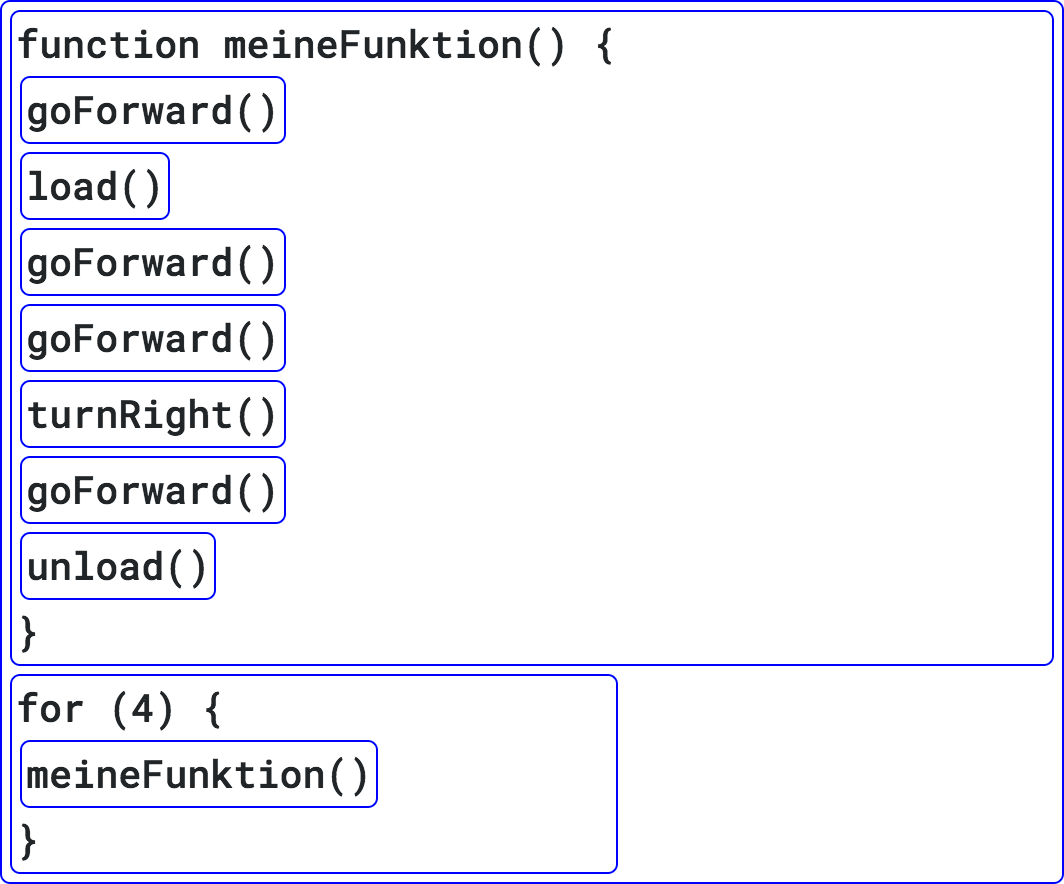
\includegraphics[width=\textwidth]{gfx/exercises-program-4.png}
    \caption{Musterlösung zu Aufgabe 4}
  \end{subfigure}\hfill
  \caption{Welt und Musterlösung zu Aufgabe 4}
\end{figure}

\pagebreak

\section{Aufgabe 5}
\label{sec:exercises:5}

Was passiert, wenn Du nicht weißt, wie oft Du Deine Prozedur ausführen musst? Benutze Sensoren und eine abweisende Schleife, um Deine Prozedur mehrmals auszuführen. Teste Dein Programm mit Welt B, C und D.

\begin{description}[noitemsep]
  \item[Welt wählen:] Welt B, Welt C, Welt D
  \item[Du brauchst:] Befehle, eigene Prozeduren, Sensoren, abweisende Schleife
  \item[Video:] \url{https://vimeo.com/315545914} (Passwort: trucklino)
\end{description}

\begin{figure}[H]
  \begin{subfigure}[b]{0.40\textwidth}
    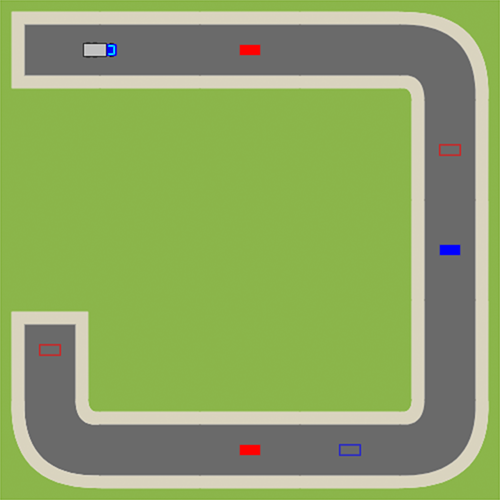
\includegraphics[width=\textwidth]{gfx/exercises-world-d.png}
    \caption{Welt D}
  \end{subfigure}\hfill
  \begin{subfigure}[b]{0.40\textwidth}
    \includegraphics[width=\textwidth]{gfx/exercises-program-5.png}
    \caption{Musterlösung zu Aufgabe 5}
  \end{subfigure}\hfill
  \caption{Welt und Musterlösung zu Aufgabe 5}
\end{figure}

\pagebreak

\section{Aufgabe 6}
\label{sec:exercises:6}

Statt einer abweisenden Schleife kannst Du auch Rekursion benutzen. Benutze eine Verzweigung, um Deine Prozedur im richtigen Moment zu verlassen.

\begin{description}[noitemsep]
  \item[Welt wählen:] Welt B, Welt C, Welt D
  \item[Du brauchst:] Befehle, eigene Prozeduren, Sensoren, Verzweigungen
  \item[Video:] \url{https://vimeo.com/315545989} (Passwort: trucklino)
\end{description}

\begin{figure}[H]
  \begin{subfigure}[b]{0.40\textwidth}
    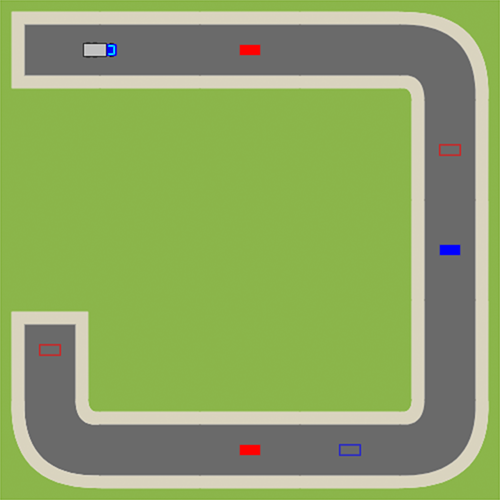
\includegraphics[width=\textwidth]{gfx/exercises-world-d.png}
    \caption{Welt D}
  \end{subfigure}\hfill
  \begin{subfigure}[b]{0.40\textwidth}
    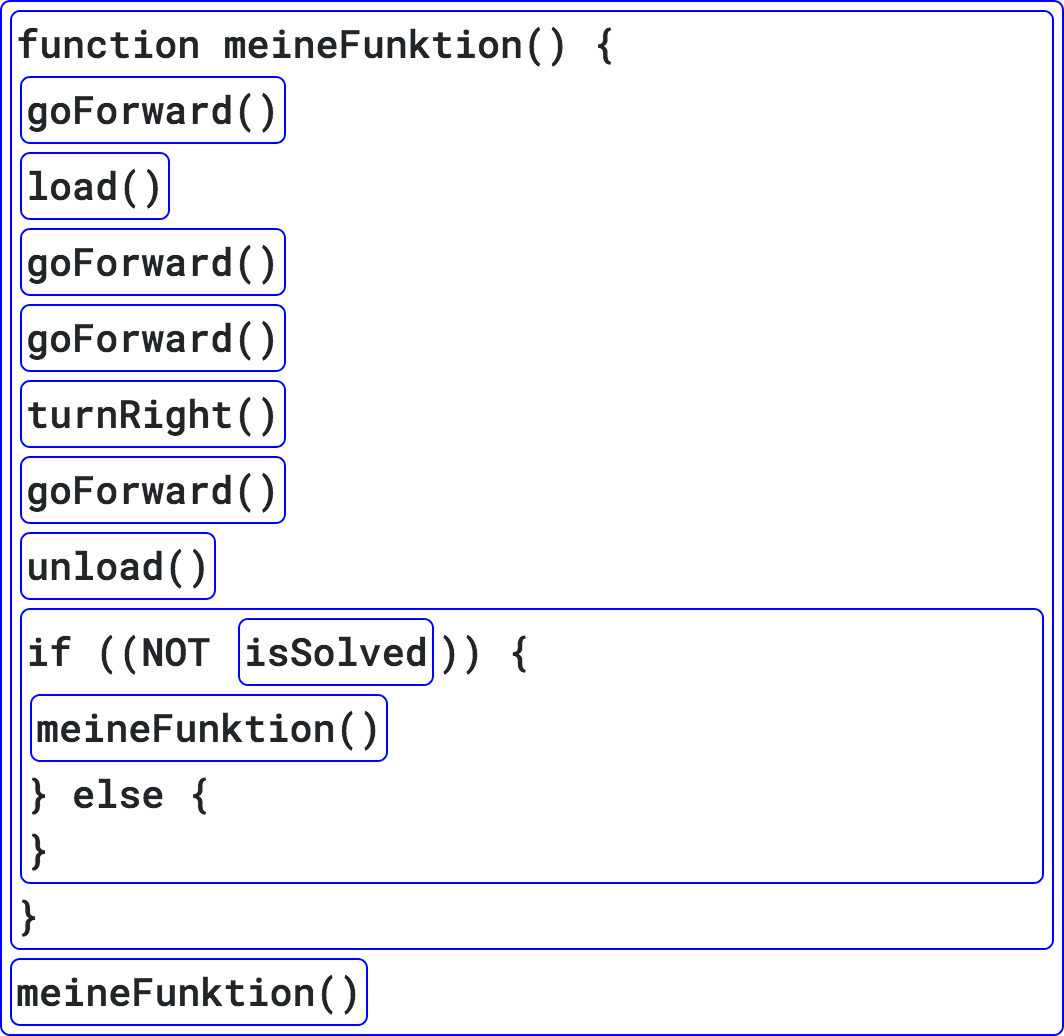
\includegraphics[width=\textwidth]{gfx/exercises-program-6.png}
    \caption{Musterlösung zu Aufgabe 6}
  \end{subfigure}\hfill
  \caption{Welt und Musterlösung zu Aufgabe 6}
\end{figure}

\pagebreak

\section{Aufgabe 7}
\label{sec:exercises:7}

Baue eine eigene Prozedur, die nicht nur geradeaus, sondern auch durch Kurven fahren kann. Deine Prozedur kannst Du solange aufrufen, bis Du am Ziel bist. Benutze dafür entweder eine abweisende Schleife oder Rekursion. Wenn Dein Programm mit Welt E funktioniert, probiere auch Welt F aus.

\begin{description}[noitemsep]
  \item[Welt wählen:] Welt E, Welt F
  \item[Du brauchst:] Befehle, eigene Prozeduren, Sensoren, Verzweigungen, abweisende Schleife (optional)
  \item[Video:] \url{https://vimeo.com/315546116} (Passwort: trucklino)
\end{description}

\begin{figure}[H]
  \begin{subfigure}[b]{0.40\textwidth}
    \includegraphics[width=\textwidth]{gfx/exercises-world-e.png}
    \caption{Welt E}
  \end{subfigure}\hfill
  \begin{subfigure}[b]{0.40\textwidth}
    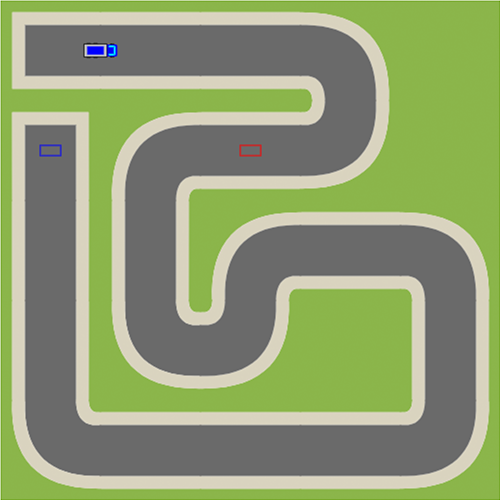
\includegraphics[width=\textwidth]{gfx/exercises-world-f.png}
    \caption{Welt F}
  \end{subfigure}\hfill
  \vspace{0.5cm}
  \begin{subfigure}[b]{0.40\textwidth}
    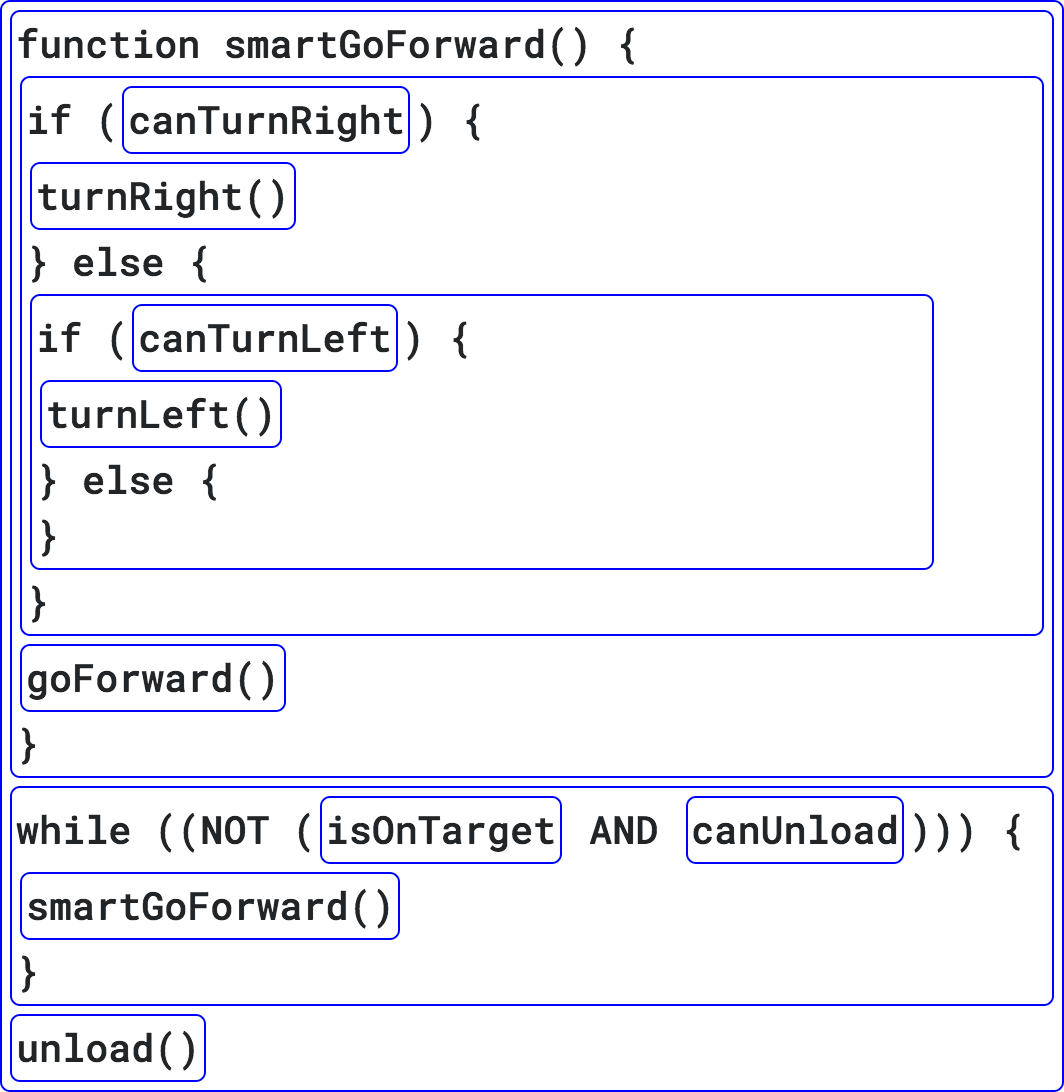
\includegraphics[width=\textwidth]{gfx/exercises-program-7.png}
    \caption{Musterlösung zu Aufgabe 7}
  \end{subfigure}\hfill
  \caption{Welten und Musterlösung zu Aufgabe 7}
\end{figure}

\pagebreak

\section{Aufgabe 8}
\label{sec:exercises:8}

Auf dem Weg sind nun einige Ampeln. Baue Dir eine zusätzliche Prozedur, die wartet, bis es grün wird.

\begin{description}[noitemsep]
  \item[Welt wählen:] Welt G
  \item[Du brauchst:] Befehle, eigene Prozeduren, Sensoren, Verzweigungen, abweisende Schleife (optional)
  \item[Video:] \url{https://vimeo.com/315546210} (Passwort: trucklino)
\end{description}

\begin{figure}[H]
  \begin{subfigure}[b]{0.40\textwidth}
    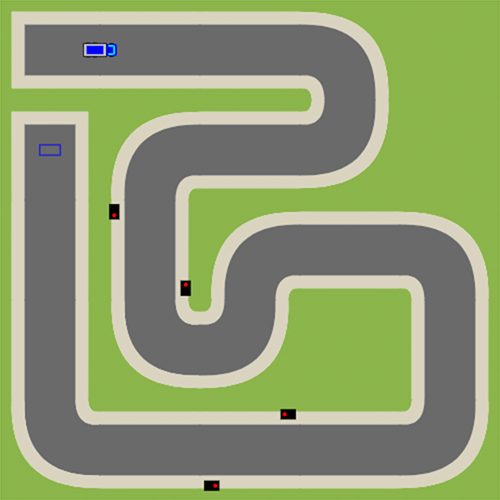
\includegraphics[width=\textwidth]{gfx/exercises-world-g.png}
    \caption{Welt G}
  \end{subfigure}\hfill
  \begin{subfigure}[b]{0.40\textwidth}
    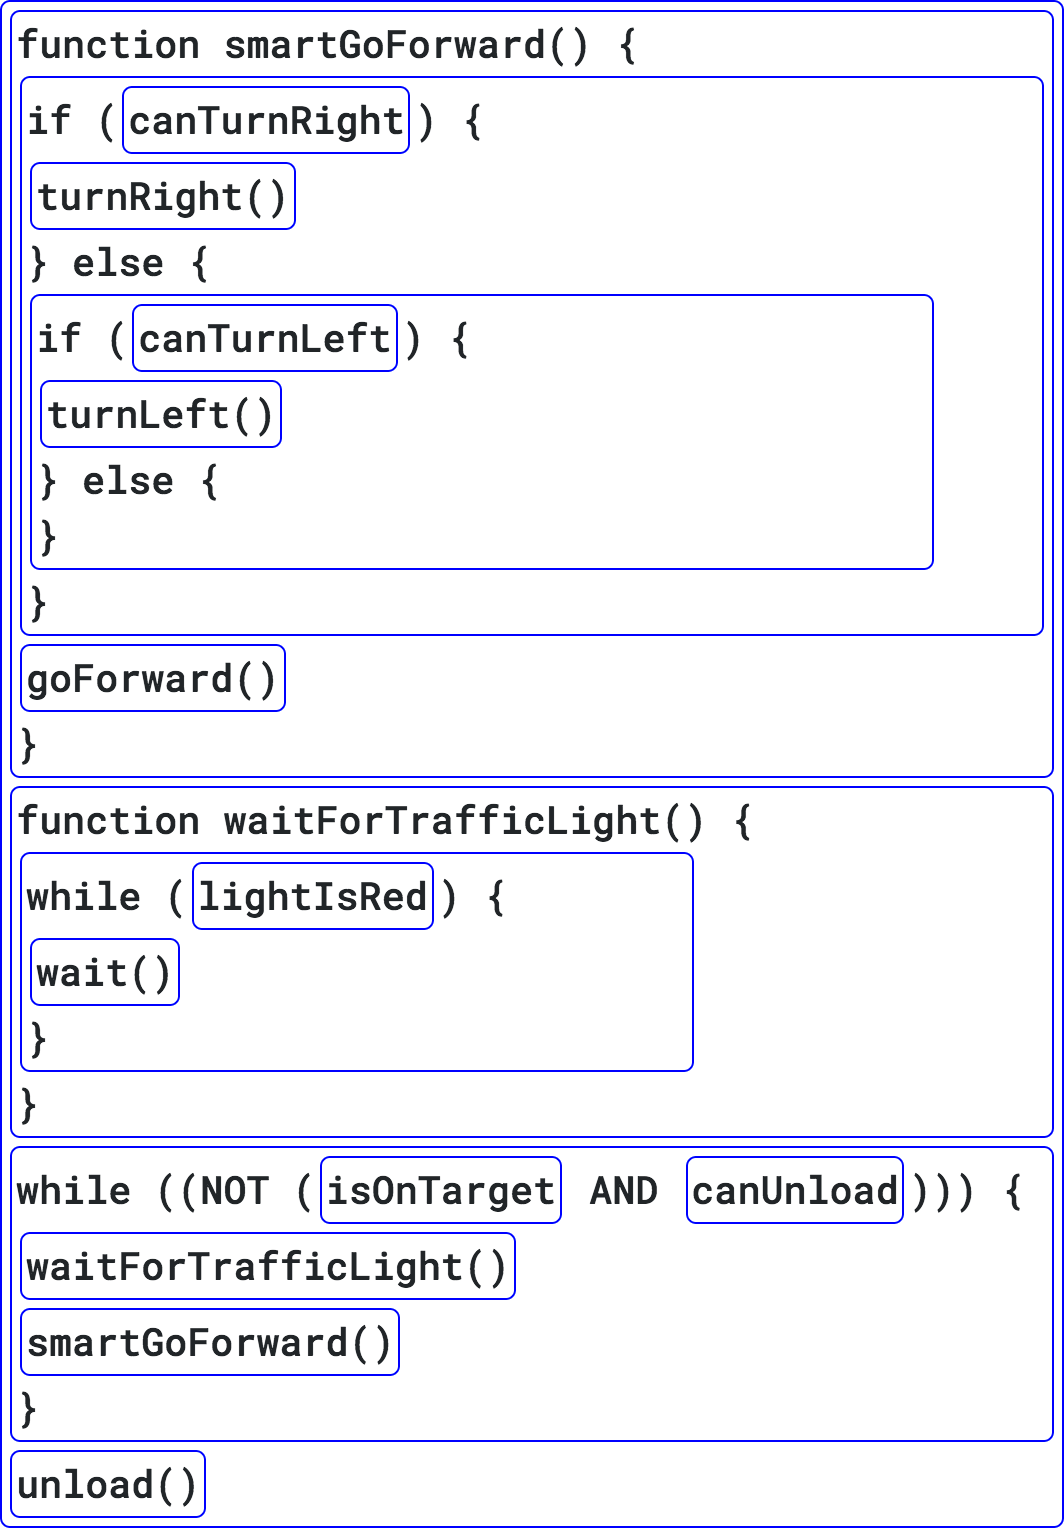
\includegraphics[width=\textwidth]{gfx/exercises-program-8.png}
    \caption{Musterlösung zu Aufgabe 8}
  \end{subfigure}\hfill
  \caption{Welt und Musterlösung zu Aufgabe 8}
\end{figure}

%%************************************************
% CD-ROM
%************************************************
\chapter{CD-ROM}
\label{sec:cd-rom}

Alle auf der beigefügten CD-ROM enthaltenen Daten sind auch im BlattWerkzeug-Git-Repository unter \url{http://blattwerkzeug.de/forward/git-repository} verfügbar.


% \listoffigures
% \cleardoublepage

% \listoftables
% \cleardoublepage

%************************************************
% Declaration
%************************************************
% \pdfbookmark[0]{Eidesstattliche Erklärung}{Eidesstattliche Erklärung}
\chapter{Eidesstattliche Erklärung}
\label{sec:declaration}
\thispagestyle{empty}

Ich erkläre hiermit an Eides statt, dass ich die vorliegende Arbeit selbstständig und ohne Benutzung anderer als der angegebenen Hilfsmittel angefertigt habe; die aus fremden Quellen direkt oder indirekt übernommenen Gedanken sind als solche kenntlich gemacht. Die Arbeit wurde bisher in ähnlicher Form keiner anderen Prüfungskommission vorgelegt und auch nicht veröffentlicht.

\bigskip
\bigskip
\bigskip
\bigskip

\begin{multicols}{2}
    \raggedright
    \thesisUniversityCity, \thesisDate

    \raggedleft
    \thesisAuthor
\end{multicols}

\cleardoublepage
